% Options for packages loaded elsewhere
\PassOptionsToPackage{unicode}{hyperref}
\PassOptionsToPackage{hyphens}{url}
%
\documentclass[
  a4paper,
]{scrbook}

\usepackage{amsmath,amssymb}
\usepackage{setspace}
\usepackage{iftex}
\ifPDFTeX
  \usepackage[T1]{fontenc}
  \usepackage[utf8]{inputenc}
  \usepackage{textcomp} % provide euro and other symbols
\else % if luatex or xetex
  \usepackage{unicode-math}
  \defaultfontfeatures{Scale=MatchLowercase}
  \defaultfontfeatures[\rmfamily]{Ligatures=TeX,Scale=1}
\fi
\usepackage{lmodern}
\ifPDFTeX\else  
    % xetex/luatex font selection
  \setmainfont[]{Latin Modern Roman}
  \setsansfont[]{Latin Modern Roman}
\fi
% Use upquote if available, for straight quotes in verbatim environments
\IfFileExists{upquote.sty}{\usepackage{upquote}}{}
\IfFileExists{microtype.sty}{% use microtype if available
  \usepackage[]{microtype}
  \UseMicrotypeSet[protrusion]{basicmath} % disable protrusion for tt fonts
}{}
\makeatletter
\@ifundefined{KOMAClassName}{% if non-KOMA class
  \IfFileExists{parskip.sty}{%
    \usepackage{parskip}
  }{% else
    \setlength{\parindent}{0pt}
    \setlength{\parskip}{6pt plus 2pt minus 1pt}}
}{% if KOMA class
  \KOMAoptions{parskip=half}}
\makeatother
\usepackage{xcolor}
\setlength{\emergencystretch}{3em} % prevent overfull lines
\setcounter{secnumdepth}{5}
% Make \paragraph and \subparagraph free-standing
\ifx\paragraph\undefined\else
  \let\oldparagraph\paragraph
  \renewcommand{\paragraph}[1]{\oldparagraph{#1}\mbox{}}
\fi
\ifx\subparagraph\undefined\else
  \let\oldsubparagraph\subparagraph
  \renewcommand{\subparagraph}[1]{\oldsubparagraph{#1}\mbox{}}
\fi


\providecommand{\tightlist}{%
  \setlength{\itemsep}{0pt}\setlength{\parskip}{0pt}}\usepackage{longtable,booktabs,array}
\usepackage{calc} % for calculating minipage widths
% Correct order of tables after \paragraph or \subparagraph
\usepackage{etoolbox}
\makeatletter
\patchcmd\longtable{\par}{\if@noskipsec\mbox{}\fi\par}{}{}
\makeatother
% Allow footnotes in longtable head/foot
\IfFileExists{footnotehyper.sty}{\usepackage{footnotehyper}}{\usepackage{footnote}}
\makesavenoteenv{longtable}
\usepackage{graphicx}
\makeatletter
\def\maxwidth{\ifdim\Gin@nat@width>\linewidth\linewidth\else\Gin@nat@width\fi}
\def\maxheight{\ifdim\Gin@nat@height>\textheight\textheight\else\Gin@nat@height\fi}
\makeatother
% Scale images if necessary, so that they will not overflow the page
% margins by default, and it is still possible to overwrite the defaults
% using explicit options in \includegraphics[width, height, ...]{}
\setkeys{Gin}{width=\maxwidth,height=\maxheight,keepaspectratio}
% Set default figure placement to htbp
\makeatletter
\def\fps@figure{htbp}
\makeatother

\usepackage{booktabs}
\usepackage{longtable}
\usepackage{array}
\usepackage{multirow}
\usepackage{wrapfig}
\usepackage{float}
\usepackage{colortbl}
\usepackage{pdflscape}
\usepackage{tabu}
\usepackage{threeparttable}
\usepackage{threeparttablex}
\usepackage[normalem]{ulem}
\usepackage{makecell}
\usepackage{xcolor}
\usepackage{fancyhdr}
\usepackage{textcomp}
\usepackage{titling}
\usepackage{pdflscape}
\usepackage{rotating}
\usepackage{geometry}
\usepackage{setspace}
\setlength{\droptitle}{-2cm}
\preauthor{
  \begin{center}
  \Large
  \vspace{15mm}
  by
  \vspace{10mm}
  
}
\postauthor{
  \end{center}
  
}

\predate{
  \begin{spacing}{1.2}
  \begin{center}
  \vspace{22mm}
  
  A thesis \\
  submitted to the Victoria University of Wellington \\
  in partial fulfilment of the requirements for the  \\
  degree of Doctor of Philosophy\\               % Degree
  \vspace{24mm}
  Te Herenga Waka $-$ Victoria University of Wellington\\
}
\postdate{
  \\
  \includegraphics[width=3in,height=1.5in]{figures/VUW-logo.png}\\
  \end{center}
  \end{spacing}
  }

\renewcommand{\topfraction}{.8}
\renewcommand{\bottomfraction}{.7}
\renewcommand{\textfraction}{.15}
\renewcommand{\floatpagefraction}{.8}
\setcounter{topnumber}{3}
\setcounter{bottomnumber}{3}
\setcounter{totalnumber}{4}

\clubpenalty=9996
\widowpenalty=9999
\makeatletter
\makeatother
\makeatletter
\@ifpackageloaded{bookmark}{}{\usepackage{bookmark}}
\makeatother
\makeatletter
\@ifpackageloaded{caption}{}{\usepackage{caption}}
\AtBeginDocument{%
\ifdefined\contentsname
  \renewcommand*\contentsname{Table of contents}
\else
  \newcommand\contentsname{Table of contents}
\fi
\ifdefined\listfigurename
  \renewcommand*\listfigurename{List of Figures}
\else
  \newcommand\listfigurename{List of Figures}
\fi
\ifdefined\listtablename
  \renewcommand*\listtablename{List of Tables}
\else
  \newcommand\listtablename{List of Tables}
\fi
\ifdefined\figurename
  \renewcommand*\figurename{Figure}
\else
  \newcommand\figurename{Figure}
\fi
\ifdefined\tablename
  \renewcommand*\tablename{Table}
\else
  \newcommand\tablename{Table}
\fi
}
\@ifpackageloaded{float}{}{\usepackage{float}}
\floatstyle{ruled}
\@ifundefined{c@chapter}{\newfloat{codelisting}{h}{lop}}{\newfloat{codelisting}{h}{lop}[chapter]}
\floatname{codelisting}{Listing}
\newcommand*\listoflistings{\listof{codelisting}{List of Listings}}
\makeatother
\makeatletter
\@ifpackageloaded{caption}{}{\usepackage{caption}}
\@ifpackageloaded{subcaption}{}{\usepackage{subcaption}}
\makeatother
\makeatletter
\@ifpackageloaded{tcolorbox}{}{\usepackage[skins,breakable]{tcolorbox}}
\makeatother
\makeatletter
\@ifundefined{shadecolor}{\definecolor{shadecolor}{rgb}{.97, .97, .97}}
\makeatother
\makeatletter
\makeatother
\makeatletter
\makeatother
\ifLuaTeX
  \usepackage{selnolig}  % disable illegal ligatures
\fi
\usepackage[citestyle = ieee,urldate = iso8601]{biblatex}
\addbibresource{references.bib}
\IfFileExists{bookmark.sty}{\usepackage{bookmark}}{\usepackage{hyperref}}
\IfFileExists{xurl.sty}{\usepackage{xurl}}{} % add URL line breaks if available
\urlstyle{same} % disable monospaced font for URLs
\hypersetup{
  pdftitle={Developing an Insect Odorant Receptor Bioelectronic Nose for Vapour-Phase Detection},
  pdfauthor={Eddyn Oswald Perkins Treacher},
  hidelinks,
  pdfcreator={LaTeX via pandoc}}

\title{Developing an Insect Odorant Receptor Bioelectronic Nose for
Vapour-Phase Detection}
\author{Eddyn Oswald Perkins Treacher}
\date{Dec 2024}

\begin{document}
\frontmatter

\maketitle

\begin{spacing}{1.2}

\clearpage
\newpage
\thispagestyle{empty} % Hide header and footer on this page
\mbox{~}
\clearpage
\newpage

%----------------------------------------------
%   Abstract
%----------------------------------------------

\thispagestyle{plain}

\begin{flushleft}
% Manually add a section to the table of contents
\pagenumbering{roman}
\addcontentsline{toc}{chapter}{Abstract}
\huge\textbf{Abstract}
\end{flushleft}

\vspace*{\baselineskip}

The ability to detect volatile organic compounds in a highly sensitive and selective manner could be used for applications as varied as diagnoses of illnesses at a remote clinic, monitoring of air in an industrial setting, or identification of invasive organisms at a biosecurity checkpoint. Historically, animal noses have been used for such tasks, as their combined sensitivity and selectivity are superior to traditional artificial sensors. However, training and deploying animals in such situations is both time and cost intensive. In recent years, an improved understanding of \textit{in vivo} biological sensing has driven efforts to mimic these highly efficient processes in an artificial sensor format. \\[5pt] To this end, a ``bioelectronic nose'' was developed. This sensor uses an artificial transducer to amplify responses of an insect odorant receptor protein to specific volatile compounds. Thin-film transistors were used as the amplifier element, given their low cost, small size and extreme sensitivity. Various thin-film morphologies were compared, and their suitability for bioelectronic nose development assessed. Transducers made using a novel steam-assisted thin-film deposition technique were found to have highly consistent device-to-device electrical properties relative to other films. Films made using this process typically showed more surface contamination than other morphologies, but their high sensitivity was confirmed with a non-specific sensing series in an aqueous environment. \\[5pt] One of the major challenges encountered in this thesis was variability in the quality of sensor functionalisation. Raman spectroscopy and fluorescence microscopy were used to confirm an existing non-covalent attachment method could successfully immobilise nanodiscs onto the transistor channel region. However, various sensors functionalised using the same procedure often exhibited no sensing activity. Extensive electrical characterisation indicated the presence of an unidentified contamination layer which prevented electrical interaction between the insect odorant receptors and the transducer thin-film. It was shown that this layer was unlikely to be directly associated with the thin-film morphology used for the transducer. \\[5pt] Subsequently, an alternative biotin-based non-covalent method was used for functionalisation of the proteins, which eliminated several possible sources of contamination. This alternative biotin-based method was used to demonstrate successful aqueous sensing \newpage
\fancyhf{} %clear all headers and footers fields
\thispagestyle{fancy} % Change header and footer on this page
\renewcommand{\headrulewidth}{0pt}
\fancyhead[L]{\textit{Abstract}} % Set header content
\fancyfoot[L]{\thepage} %prints the page number on the left side of the header
of femtomolar concentrations of methyl salicylate by an iOR10a-functionalised device. When tested in a custom-built vapour delivery system, a similar bioelectronic sensor was shown to be highly sensitive to the target vapour. However, consistent reproduction of the biotin-based method was challenging due to the harsh cleaning method involved. It was therefore difficult to determine conclusively whether the vapour-phase sensor responses were selective. By finding new, systematic approaches to address the barriers to sensor success carefully identified in this work, there are promising signs that a highly reliable vapour-phase bioelectronic nose can be produced.

\clearpage
\newpage

%----------------------------------------------
%   Acknowledgement
%----------------------------------------------

\thispagestyle{plain}

\begin{flushleft}
% Manually add a section to the table of contents
\addcontentsline{toc}{chapter}{Acknowledgements}
\huge\textbf{Acknowledgements}
\end{flushleft}

\vspace*{\baselineskip}

I would first like to acknowledge the lands of my ancestors, and the lands of the sovereign first peoples to which my ancestors travelled. We each come from the land, live off the land and return to the land.
\end{spacing}
\begin{spacing}{1.2} 
\textit{Noon of Essex to Warrang, on the Friends, Autumn 1811} \\[5pt]
\textit{Cave of Cambridgeshire to Warrang, on the Royal Charlotte, Autumn 1825} \\[5pt]
\textit{Boyce of Suffolk to Warrang, 1832} \\[5pt] 
\textit{Charlton of Northumberland to Warrang, on the Clyde, Spring 1834} \\[5pt]
\textit{Prouse of Devonshire to Pito-one, on the Duke of Roxburgh, Summer 1840} \\[5pt]
\textit{Ebden of Devonshire to Pito-one, on the Tyne, Winter 1841} \\[5pt]
\textit{Collis of Hampshire to Pito-one, on the Birman, Autumn 1842} \\[5pt]
\textit{Swann of Loch Garman to Te Whanganui-a-Tara, 1844} \\[5pt] 
\textit{Blythe of Berkshire to Whakatū, circa 1846} \\[5pt]
\textit{Innes of Berkshire to Naarm, on the Sacramento, Autumn 1853} \\[5pt]
\textit{Sheppard of Gloucestershire to Naarm, 1853} \\[5pt] 
\textit{Bruce of London to Naarm, on the Omega, Autumn 1855} \\[5pt]
\textit{Quennell of Surrey to Warrang, on the Asiatic, Winter 1855} \\[5pt]
\textit{Barr of Glasgow to Kōpūtai, on the Sir Edward Paget, Winter 1856} \\[5pt] 
\textit{Perkins of London to Te Whanganui-a-Tara, on the Matoaka, Spring 1859} \\[5pt]
\textit{McKee of Antrim to Tāmaki Makaurau, on the Indian Empire, Spring 1862} \\[5pt]
\textit{Sandilands of Peeblesshire to Ōtepoti, circa 1864} \\[5pt] 
\textit{Treacher of Berkshire to Te Whanganui-a-Tara, on the Wild Duck, Summer 1865} \\[5pt]
\textit{McTaggart of Argyllshire to Kōpūtai, on the Edward P. Bouverie, Autumn 1869} \\[5pt] 
\textit{Chapman of Kent to Whakatū, on the Adamant, Winter 1874} \\[5pt]
\textit{Cheel of London to Whakatū, on the Queen Bee, Winter 1877} \\[5pt]  
\textit{Hutchison of Aberdeen to Tarntanya, before 1882.}
\end{spacing}
\begin{spacing}{1.2} 
\newpage
\fancyhf{} %clear all headers and footers fields
\thispagestyle{fancy} % Change header and footer on this page
\renewcommand{\headrulewidth}{0pt}
\fancyhead[L]{\textit{Acknowledgements}} % Set header content
\fancyfoot[L]{\thepage} %prints the page number on the left side of the header 
I chose to start my doctoral studies just a few months into a global pandemic. Completing a challenging project with a worldwide crisis in the background might have been impossible without the supervision of AProf. Natalie Plank. Her ability to adapt to and overcome any problem has taught me that there is no situation which is truly unmanageable. I am deeply grateful for her leadership throughout a time of particular chaos. \\[5pt] I started this project with minimal formal training in biological science, coming from a primarily physics and engineering background. The immense support I received from Melissa Jordan and Colm Carraher from the Institute for Plant and Food Research (PFR) to complete this project meant that this was not an issue, and I thank them both for this. \\[5pt] I would not have been able to begin this thesis without the financial backing and support I received from PFR and the Better Border Biosecurity (B3) programme. In particular, I am very grateful to Andrew Kralicek, formerly with PFR and now at Scentian Bio, and the ex-Director of B3, David Teulon, for helping to secure funding for my project. I would also like to thank the donor of the Ernest Marsden Scholarship in Physics for their significant financial support. \\[5pt] There are many incredibly supportive people who I worked alongside during my project. I would like to start off by thanking Rifat Ullah, whose mentoring and kindness encouraged me to pursue further study. His work on the initial design and setup of the vapour delivery system was invaluable to me throughout this project. I am also especially grateful to Alex Puglisi, for constructing the mechanical elements of the vapour delivery system and giving me extensive feedback on the system design. I would like to thank Peter Coard, for his advice and guidance when constructing the electrical elements of the vapour delivery system. I thank Selvan Murugathas, too, for his advice on constructing the insect odorant receptor sensors, as well as Damon Colbert and Valentina Lucarelli, who provided the insect odorant receptor nanodiscs used in this work. \\[5pt] Thank you to Prof. Ben Ruck, my supportive secondary supervisor, and to AProf. Franck Natali, for always asking about my thesis in the tearoom. Thank you to Gideon Gouws for his friendly encouragement and advice. For their substantial technical assistance and mentoring during this project, I thank Alan Rennie, Grant Franklin, Chris Lepper, Rashika Gunasekara, Pete Jebson and Sushila Pillai from VUW, Andrew Chan from PFR, AProf. Charles Unsworth from the University of Auckland, and Prof. Simon Brown and his nanomaterials group from the University of Canterbury. \\[5pt] I was lucky enough to start my doctoral program just as a group of supportive and talented senior students were finishing, and finished just as a group of enthusiastic and talented new doctoral students were starting. A special thanks to Jenna Nyugen, Erica Happe and Erica Cassie for teaching me the fabrication processes and characterisation procedures that made this thesis happen; and a special thanks to Marissa Dierkes, Danica Fontein, Sangar Begzaad and Alireza Zare, for their incredible support throughout the thesis writing process. I am also thankful for the assistance of the cleanroom group interns over the course of my PhD, including Liam, Hayden and Lotte. I would further like to thank everyone else I shared an office with and worked alongside, including Jackson, Will, Roshni, Ali, Sam, Kira, Catherine, Martin, Janani, Ted, Kiri and Joe. \\[5pt] A massive thank you to Openstar Technologies. It has been an honour to work on a cutting-edge plasma physics project right here in Te Whanganui-a-Tara. A particularly big thank you to Ratu, Darren and Thomas for having me as part of the plasma physics team. Thank you also to the other Openstar interns, in particular the other plasma physics interns, Valentina, Benjy and Chris. I wish you success in all your dipole-confined plasma related endeavours. \\[5pt] I want to thank Shodokan Aikido New Zealand for their support throughout this thesis, in particular for the once-in-a-lifetime opportunity to travel to Osaka to be graded for first-dan by Nariyama Shihan. Thanks for all the training and support, Ian. \\[5pt] Thank you to all the friends and whānau, old and new, who have supported me over these wild past few years. You know who you are. \\[5pt] Thank you to my brother, Keeson, and to my parents, Hilary and Phillip. Your support means everything to me, and I would not be where I am today without you. Our Friday lunchtime cafe visits kept me motivated and inspired throughout the doctoral program. Thank you, thank you, thank you for your love, your compassion, and for being there for me. \\[5pt] Finally, thank you Nina. Your incredible love has kept me going through the most difficult and most wonderful times over the last four years. You are the light of my life, and I am so happy to have taken on this challenge with you by my side. \\[5pt] Arohanui and peace to you all, Eddyn (Ned)

\fancyhf{} %clear all headers and footers fields
\thispagestyle{fancy} % Change header and footer on this page
\renewcommand{\headrulewidth}{0pt}
\fancyhead[R]{\textit{Acknowledgements}} % Set header content
\fancyfoot[R]{\thepage} %prints the page number on the right side of the header

\clearpage
\newpage
\thispagestyle{empty} % Hide header and footer on this page
\mbox{~}
\clearpage
\newpage

\pagestyle{headings}

\end{spacing}\ifdefined\Shaded\renewenvironment{Shaded}{\begin{tcolorbox}[boxrule=0pt, breakable, enhanced, borderline west={3pt}{0pt}{shadecolor}, sharp corners, frame hidden, interior hidden]}{\end{tcolorbox}}\fi

\begin{spacing}{1.2}

\renewcommand*\contentsname{Table of Contents}
{
\setcounter{tocdepth}{2}
\addcontentsline{toc}{chapter}{Table of Contents}
\tableofcontents
}
\listoffigures
\addcontentsline{toc}{chapter}{List of Figures}
\listoftables
\addcontentsline{toc}{chapter}{List of Tables}

\clearpage
\newpage

%----------------------------------------------
%   List of Abbreviations
%----------------------------------------------

\thispagestyle{plain}

\begin{flushleft}
% Manually add a section to the table of contents
\addcontentsline{toc}{chapter}{List of Abbreviations}
\huge\textbf{List of Abbreviations}
\end{flushleft}

\vspace*{\baselineskip}

\begin{table}[H]
  \begin{tabular}{@{}p{0.25\textwidth} p{0.75\textwidth}@{}}  % Adjust the width as needed
    2D  & 2-Dimensional  \\[5pt]
    Ab  & Antibody  \\[5pt]
    AB  & Amyl Butyrate  \\[5pt]
    AB-NTA  & N$\alpha$,N$\alpha$-Bis(carboxymethyl)-\textit{L}-lysine hydrate  \\[5pt]
    AFM  & Atomic Force Microscope/Microscopy  \\[5pt]
    AH  & Absolute Humidity  \\[5pt]
    Avi-tag  & Avidin-tag  \\[5pt]
    BMIM  & 1-butyl-3-methylimidazolium bis(trifluoromethylsulfonyl)imide  \\[5pt]
    BWF  & Breit-Wigner-Fano  \\[5pt]
    CAD  & Computer Aided Design \\[5pt]
    CNT  & Carbon Nanotube  \\[5pt]
    CVD  & Chemical Vapour Deposition  \\[5pt]
    Cy3  & Cyanine 3  \\[5pt]
    DAN  & 1,5-diaminonaphthalene  \\[5pt]
    DAQ  & Data Acquisition Input/Output Module  \\[5pt]
    DCB  & 1,2-dichlorobenzene  \\[5pt]
    DI  & Deionised  \\[5pt]
    DMF  & Dimethylformamide   \\[5pt]
    DMSO  & Dimethylsulfoxide   \\[5pt]
    DMT-MM   & 4-(4,6-dimethoxy-1,3,5-triazin-2-yl)-4 methylmorpholinium chloride \\[5pt]
    DMMP  & Dimethyl Methylphosphonate  \\[5pt]
    DNA  & Deoxyribonucleic Acid  \\[5pt]
    E2Hex  & \textit{trans}-2-hexan-1-al  \\[5pt]
    EB  & Ethyl Butyrate  \\[5pt]
  \end{tabular}
\end{table}

\newpage
\fancyhf{} %clear all headers and footers fields
\thispagestyle{fancy} % Change header and footer on this page
\renewcommand{\headrulewidth}{0pt}
\fancyhead[L]{\textit{List of Abbreviations}} % Set header content
\fancyfoot[L]{\thepage} %prints the page number on the right side of the header
\begin{table}[H]
  \begin{tabular}{@{}p{0.25\textwidth} p{0.75\textwidth}@{}}  % Adjust the width as needed
    EDC  & 1-Ethyl-3-(3-dimethylaminopropyl)carbodiimide  \\[5pt]
    EDL  & Electric Double Layer  \\[5pt]
    EIS  & Electrochemical Impedance Spectroscopy  \\[5pt]
    EtHex  & Ethyl Hexanoate  \\[5pt]
    EtOH  & Ethanol  \\[5pt]
    FET  & Field-Effect Transistor  \\[5pt]
    FITC  & Fluorescein isothiocyanate  \\[5pt]
    GA  & Glutaraldehyde  \\[5pt]
    GFET  & Graphene Field-Effect Transistor  \\[5pt]
    GFP  & Green Fluorescent Protein  \\[5pt]
    GPCR  & G-protein Coupled Receptor  \\[5pt]
    HEK  & Human Embryonic Kidney  \\[5pt]
    His-tag  & Histidine-tag  \\[5pt]
    hOR  & Human Odorant Receptor  \\[5pt]
    HPLC  & High-performance Liquid Chromatography   \\[5pt]
    iOR  & Insect Odorant Receptor  \\[5pt]
    IPA  & Isopropanol  \\[5pt]
    LOD  & Limit of Detection  \\[5pt]
    m-CNT  & Metallic Carbon Nanotube   \\[5pt]
    MeOH  & Methanol   \\[5pt]
    MeSal  & Methyl Salicylate   \\[5pt]
    MFC  & Mass Flow Controller   \\[5pt]
    mOR  & Mouse Odorant Receptor  \\[5pt]
    MOSFET  & Metal-Oxide-Semiconductor Field-Effect Transistor  \\[5pt]
    MSP  & Membrane Scaffold Protein  \\[5pt]
    MWCNT  & Multi-Walled Carbon Nanotube  \\[5pt]
    ND  & Nanodisc  \\[5pt]
  \end{tabular}
\end{table}

\newpage
\fancyhf{} %clear all headers and footers fields
\thispagestyle{fancy} % Change header and footer on this page
\renewcommand{\headrulewidth}{0pt}
\fancyhead[R]{\textit{List of Abbreviations}} % Set header content
\fancyfoot[R]{\thepage} %prints the page number on the right side of the header
\begin{table}[H]
  \begin{tabular}{@{}p{0.25\textwidth} p{0.75\textwidth}@{}}  % Adjust the width as needed
    NHS  & N-Hydroxysuccinimide  \\[5pt]
    NHSS  & N-hydroxysulfosuccinimide   \\[5pt]
    NMR  & Nuclear Magnetic Resonance  \\[5pt]
    NSB  & Non-Specific Binding   \\[5pt]
    NTA  & Nitrilotriacetic Acid   \\[5pt]
    OBP  & Odorant Binding Protein  \\[5pt]
    OR  & Odorant Receptor  \\[5pt]
    ORCO  & Odorant Receptor Co-Receptor  \\[5pt]
    PBA  & 1-Pyrenebutyric Acid  \\[5pt]
    PBASE  & 1-Pyrenebutanoic Acid N-hydroxysuccinimide Ester  \\[5pt]
    PBS  & Phosphate-Buffered Saline  \\[5pt]
    PCB  & Printed Circuit Board   \\[5pt]
    PDL & Poly-\textit{D}-lysine  \\[5pt]
    PDMS  & Polydimethylsiloxane   \\  [5pt]
    PEG  & Polyethylene Glycol  \\[5pt] 
    PID  & Photoionisation Detector  \\[5pt]
    P\&ID & Process \& Instrumentation Diagram  \\[5pt]
    PLL  & Poly-\textit{L}-lysine  \\[5pt]
    PPB  & Pyrene-PEG-Biotin  \\[5pt]
    PPF  & Pyrene-PEG-FITC  \\[5pt]
    PPN  & Pyrene-PEG-NTA  \\[5pt]
    PPR  & Pyrene-PEG-Rhodamine  \\[5pt]
    PTFE  & Polytetrafluoroethylene (Teflon™)  \\[5pt]
    PVC  & Polyvinyl chloride  \\[5pt]
    QCM  & Quartz Crystal Microbalance  \\[5pt]
    RH  & Relative Humidity  \\[5pt]
    RHI  & Relative Humidity and Temperature Indicator  \\[5pt] 
  \end{tabular}
\end{table}

\newpage
\fancyhf{} %clear all headers and footers fields
\thispagestyle{fancy} % Change header and footer on this page
\renewcommand{\headrulewidth}{0pt}
\fancyhead[L]{\textit{List of Abbreviations}} % Set header content
\fancyfoot[L]{\thepage} %prints the page number on the right side of the header
\begin{table}[H]
  \begin{tabular}{@{}p{0.25\textwidth} p{0.75\textwidth}@{}}  % Adjust the width as needed
    RNA  & Ribonucleic Acid   \\[5pt]
    SAW  & Surface Acoustic Wave   \\[5pt]
    s-CNT  & Semiconducting Carbon Nanotube   \\[5pt]
    SEM  & Scanning Electron Microscope/Microscopy   \\[5pt]
    SMU  & Source Measure Unit   \\[5pt]
    SPR  & Surface Plasmon Resonance   \\[5pt]
    SWCNT  & Single-Walled Carbon Nanotube   \\[5pt]
    TFTFET  & Thin-Film Field-Effect Transistor  \\[5pt]
    TMAH  & Tetramethylammonium hydroxide  \\[5pt]
    TX  & Transfer Characteristics  \\[5pt]
    UV  & Ultraviolet  \\[5pt]
    VI  & Virtual Instrument  \\[5pt]
    VUAA1  & N-(4-Ethylphenyl)-2-{[4-ethyl-5-(pyridin-3-yl)-4H-1,2,4-triazol-3-yl]sulfanyl}acetamide  \\[5pt] 
  \end{tabular}
\end{table}

% Adjust the top and bottom margins of float pages to center floats
\makeatletter
\setlength{\@fptop}{0pt plus 1fil}
\setlength{\@fpbot}{0pt plus 1fil}
\makeatother

\fancyhf{} %clear all headers and footers fields
\thispagestyle{fancy} % Change header and footer on this page
\renewcommand{\headrulewidth}{0pt}
\fancyhead[L]{\textit{List of Abbreviations}} % Set header content
\fancyfoot[L]{\thepage} %prints the page number on the right side of the header

\clearpage
\newpage

\end{spacing}

\pagestyle{headings}
\setstretch{1.2}
\mainmatter
\bookmarksetup{startatroot}

\hypertarget{introduction}{%
\chapter{Introduction}\label{introduction}}

\hypertarget{background}{%
\section{Background}\label{background}}

The ``bioelectronic nose'', an electronic transducer modified with
elements of the animal olfactory system, has the potential to allow
specific detection of airborne volatile compounds at concentrations as
low as parts per trillion
\autocite{Glatz2011,Kwon2015,Dung2018,Kim2022a}. The thin-film
transistor (TFT), a type of field-effect transistor (FET), is a
particularly portable, simple to use, small and robust option for the
transducer component \autocite{Kauffman2008,Khan2020}. The thin films
used in these transistors include carbon nanotube networks and graphene,
low-dimensional nanomaterials which are both highly sensitive and
biocompatible \autocite{Shkodra2021}. The implications of successful
development of such a portable and robust bioelectronic nose are
significant. Applications could be found in high-importance fields such
as biosecurity, medicine, environmental protection and food safety
\autocite{Dung2018,Arakawa2019,Yang2017,Son2017}. For example, it has
been demonstrated that it is possible to specifically detect invasive
brown marmorated stinkbugs based on their volatile trace
\autocite{Moser2020}. A bioelectronic nose could potentially accomplish
this biosecurity task far more cheaply and efficiently than trained
sniffer dogs \autocite{Lee2010,Moon2020,Terutsuki2020}. There has been
rapid progress in the development of bioelectronic noses using carbon
nanotube field-effect transistors (CNT FETs) and graphene field-effect
transistors (GFETs) over the past 15-20 years
\autocite{Yoon2009,Lee2010,Yang2018}.

Insect odorant receptors (iORs) enable simple invertebrates, such as the
vinegar fruit fly \emph{Drosophila melanogaster}, to distinguish between
a huge number of specific volatile compounds
\autocite{Hallem2004,Smart2008,Wicher2008,Munch2016,Bohbot2020}. Within
the past five years, a variety of \emph{Drosophila melanogaster} iORs
have been successfully coupled with highly sensitive low-dimensional
thin-film transistors for specific detection of fruit-like odors in an
aqueous environment \autocite{Murugathas2019a,Murugathas2020}. Insect
odorant receptors have also been used for sensitive and selective
volatile detection of volatile compounds in a lipid bilayer format
\autocite{Yamada2021}. In this thesis, the primary aim was to verify
whether a bioelectronic nose capable of odorant detection in a
vapour-phase environment could be constructed by coupling iORs with
thin-film transistors. Alongside the future use of this technology in
targeted sensor applications, development of a vapour-phase
bioelectronic nose using iORs may give us a greater understanding of the
mechanisms underlying insect olfaction \autocite{Lee2010}. The
transduction mechanism of nanomaterial-based iOR sensors is still
unknown, and it is hoped this work sheds further light on the biological
and electronic processes underpinning this mechanism
\autocite{Murugathas2020,Khadka2019,Cheema2021}.

To answer the question of whether selective vapour-phase detection could
be achieved using the architecture described above, it was first
important to verify that each of the component parts of this highly
integrated system functioned as expected and were mutually compatible.
As the thin-film transistor is a relatively recent technology, the
design and fabrication of these devices continues to evolve, and it was
important to ensure that the methods used gave rise to devices of
consistent quality which were sufficiently sensitive. Insect odorant
receptor biofunctionalisation is also an emerging field; it was
important to review and test existing functionalisation approaches,
identifying their relative strengths and weaknesses for biosensor
applications. Finally, to ensure that both functioning parts worked
together once integrated, the functionalised transducer was tested in an
aqueous environment to compare its sensitivity with previous research
\autocite{Murugathas2019a,Murugathas2020}. A suitable vapour delivery
system for testing the working sensors was developed in parallel, with
reference sensors installed to compare their responses with the activity
of the biosensor. Once this system was confirmed to behave in a
controllable manner, the bioelectronic nose was tested in the
vapour-phase environment.

\hypertarget{thesis-outline}{%
\section{Thesis Outline}\label{thesis-outline}}

This thesis consists of ten chapters. The first three chapters,
including this one, are background chapters introducing the general
topics of this thesis. The fourth chapter is a methods chapter,
describing device fabrication and characterisation in detail. The fifth,
sixth and seventh chapters describe the results obtained when verifying
the sensitivity of the novel biosensor in an aqueous environment, while
the eighth and ninth chapters relate the results of testing the
biosensing platform in a vapour-phase environment. The tenth chapter
concludes the thesis and discusses possible next steps for future
research.

\textbf{Chapter 2} gives a broad description of carbon nanotube and
graphene field-effect transistors with a focus on their use in sensing
applications. The chapter begins by looking at the general structure and
properties of thin-film transistors, where key figures of merit such as
transconductance, on-off ratio, gate current and hysteresis are
described. The chemical compositions of graphene and carbon nanotube
networks are discussed, as well as their conduction behaviour and unique
sensing properties when integrated into a field-effect transistor as the
thin-film element.

\textbf{Chapter 3} investigates previous odorant receptor-coupled
thin-film field-effect transistors examined in the literature. First,
the biological structure of odorant receptors and membrane formats for
their protection \emph{in vitro} are discussed. Details are then
provided regarding the construction and operation of existing vertebrate
odorant receptor biosensors. The structure and function of the insect
odorant receptor is then contrasted with the vertebrate odorant
receptor, and existing insect odorant receptor TFT biosensors in the
literature are discussed. The chapter finishes with a brief discussion
of non-specific binding and its role in hindering biosensor activity.

\textbf{Chapter 4} describes the fabrication of the CNT FET and GFET
transducers used in this thesis and the characterisation techniques used
to probe their behaviour. The chapter starts with an introduction to
photolithography for thin-film transistor device fabrication. Various
techniques are described for random deposition of carbon nanotube
networks to act as channels for these thin-film transistors.
Characterisation techniques described in this chapter include atomic
force microscopy (AFM), fluorescence microscopy, Raman spectroscopy, and
electrical characterisation with various semiconductor device analysers.

\textbf{Chapter 5} presents the results obtained from the use of
characterisation techniques on the pristine GFETs and CNT FETs. Various
carbon nanotube (CNT) network morphologies are displayed and analysed.
The Raman spectra and electrical device parameters of these CNT network
morphologies are then discussed, along with electrical parameters from
graphene devices. The sensitivity of a dense CNT network morphology
device is then verified in the aqueous phase.

\textbf{Chapter 6} explores the non-covalent functionalisation of GFETs
and CNT FETs with various linker molecules for insect odorant receptor
attachment. The linker molecules tested were 1-pyrenebutanoic acid
N-hydroxysuccinimide ester (PBASE) and 1-pyrenebutyric acid (PBA) with
1-Ethyl-3-(3-dimethylaminopropyl)carbodiimide (EDC). Pyrene-NTA and
pyrene-biotin were also investigated as other possible linker molecules.
The quality of various functionalisation approaches was then explored
with various fluorescent-tagged linker molecules and biomolecules. In
this process, various potential obstacles to successful biosensor
functionalisation were identified.

\textbf{Chapter 7} maps out progress made towards the creation of an
insect odorant receptor functionalised thin-film biosensor which is
responsive to target analyte in an aqueous environment. Two different
approaches are described that gave rise to working aqueous-phase
biosensors. The first functionalisation approach, which used PBASE in
methanol, led to results that were difficult to reproduce. Possible
factors underlying the unreliability of this method were then
investigated. A second approach was then designed to avoid the
undesirable influence of the confounding factors identified.

\textbf{Chapter 8} outlines the development of a vapour delivery system
for characterisation of the insect odorant receptor functionalised TFT
biosensors in a vapour-phase environment. The vapour delivery system was
upgraded from an existing system to include new mass flow controllers
(to have greater control of flow through the system) and off the shelf
vapour sensors (to collect vapour flow data that could be used for
comparison against biosensor activity). The chapter also describes the
design and construction of an electronic interface to monitor and
control the components of the vapour delivery system, as well as
calibration of the mass flow controllers.

\textbf{Chapter 9} details the use of the vapour delivery system for
testing the functionalised biosensors in the vapour phase. First, the
flow behaviour of volatile organic vapours through the system was
validated using onboard reference sensors. The response of a pristine
carbon nanotube device to two volatile compounds was investigated and
compared to signals from the reference sensors. Finally, a device
functionalised using the second functionalisation approach from chapter
7 was tested in the vapour delivery system, and its responses to vapour
were compared to those of a pristine device.

\textbf{Chapter 10} summarises the conclusions drawn from this work, and
proposes various related studies which can be undertaken to continue the
work described in this thesis.

\bookmarksetup{startatroot}

\hypertarget{sec-vapour-biosensing-iORs}{%
\chapter{Vapour-Phase Sensing with iOR-Functionalised Carbon Nanotube
Devices}\label{sec-vapour-biosensing-iORs}}

\hypertarget{introduction-1}{%
\section{Introduction}\label{introduction-1}}

In the previous chapter, \textbf{?@sec-vapour-sensing-biosensors}, the
development of a vapour delivery system for testing novel field-effect
transistor-based biosensors was detailed. Once the vapour delivery
system was successfully constructed and calibrated, the next step was to
use the vapour delivery system to test the response of functionalised
insect odorant receptor (iOR) biosensors to ethyl hexanoate and
\emph{trans}-2-hexenal, two odorant compounds associated with the scent
of a Queensland fruit fly infestation. A successful vapour-phase
biosensor sensitive to these compounds could be used to identify and
eliminate these potentially costly infestations
\autocite{Queensland1,Queensland2}. A variety of functionalisation
procedures were previously trialled in an aqueous environment, with the
results of these trials described in \textbf{?@sec-biosensing-iORs}. The
most successful approach, which eliminated a number of possible surface
coatings and discarded the nanodisc format, could then be tested in the
vapour delivery system. Numerous alternative functionalisation
approaches trialled in \textbf{?@sec-biosensing-iORs} were unable to
produce sensors which consistently responded to their target analyte.
The inconsistent behaviour of these sensors meant they were considered
inappropriate for testing in the vapour delivery system, as it would be
difficult to determine whether a sensor had failed to respond because
the analyte was in vapour phase, or if the functionalisation had simply
been unsuccessful.

This chapter first demonstrates that the reference sensors described in
\textbf{?@sec-vapour-sensing-biosensors} were able to non-selectively
respond to vapour in a consistent manner. These reference sensors were
then used to monitor the vapour system chamber environment during sensor
testing; the reference sensor responses were measured to ensure sensors
were responding to vapour and not to other environmental effects. Next,
measurements were taken to understand the response of pristine carbon
nanotube thin-film transistors to volatile compounds in the vapour
delivery system, to later compare with the response of functionalised
devices to similar vapour concentrations. The transducers were shown to
give a small signal response to nominal parts per million concentrations
of ethyl hexanoate and \emph{trans}-2-hexenal. A device was then
functionalised using the aqueous approach described in
\textbf{?@sec-aqueous-functionalisation}, and exposed to
\emph{trans}-2-hexenal vapour in the delivery system. However, little
response to the positive analyte was shown by the functionalised sensor
when compared to a pristine control. The chapter finishes with a
discussion of possible reasons for the lack of response to vapour shown
by the functionalised device.

\hypertarget{sec-responses-to-vapour}{%
\section{Reference Sensor Responses to Vapour
Flow}\label{sec-responses-to-vapour}}

Once the rate of flow through the device chamber had been calibrated,
the correct operation of the reference sensors used in the system was
verified. Various flow rates in and out of the chamber were used to
calibrate and verify the reference sensors. These flows in and out of
the chamber are labelled on the simplified schematic in
Figure~\ref{fig-chamber-schematic}. Note that the labels on this
schematic assume that nitrogen compression at any point within this
schematic is negligible. \textbf{?@sec-calibration} shows that a 200
sccm flow into the chamber corresponds to an actual rate for \(C + D\)
of \(\sim\) 230 sccm. If a 150 sccm flow rate as measured by the
flowmeter is pumped out through the PID, \textbf{?@sec-calibration}
shows that \(P \sim\) 110 sccm. This means that \(\sim\) 50\% of the
flow through the chamber exits via the PID. If a 100 sccm flowmeter rate
is pumped through the PID, \(P \sim\) 70 sccm, and therefore \(\sim\)
30\% of the chamber flow exits through the PID.

\begin{figure}

{\centering \includegraphics[width=1\textwidth,height=\textheight]{figures/ch9/chamber-manifold-v2.png}

}

\caption[Simplified schematic showing the flow into and out of the
device chamber and manifold of the delivery
system.]{\label{fig-chamber-schematic}Simplified schematic showing the
flow into and out of the device chamber and manifold of the delivery
system. The input flows from the carrier and dilution line are
represented by \(C\) and \(D\), and the output flow through the PID is
represented by \(P\). The exhaust can either flow past the relative
humidity indicator or straight to the fumehood. This diagram assumes
that flow through leaks in the chamber and manifold is low enough to be
considered negligible, which was confirmed by leak testing with bubble
solution.}

\end{figure}

\hypertarget{relative-humidity-indicator}{%
\subsection{Relative Humidity
Indicator}\label{relative-humidity-indicator}}

To test the relative humidity indicator (RHI), all valves out of the
chamber were sealed except for the valve of the relative humidity
indicator chamber. This meant all flow coming out of the system would
pass through the relative humidity indicator chamber (\(P\) = 0 sccm and
exhaust goes to RHI in Figure~\ref{fig-chamber-schematic}). Continuous
nitrogen flow was then placed through the chamber until relative
humidity dropped to about 20\%. 10 mL of deionised water was placed into
the analyte bottle. A series of different flow rates through each line
were sent to the chamber as shown by the purple traces in
Figure~\ref{fig-RHI-verification}. Note that between 200 s and 600 s,
the total flow rate remains the same, but the ratio of dilution flow to
carrier flow differs.

\begin{figure}

{\centering \includegraphics[width=0.65\textwidth,height=\textheight]{figures/ch9/RHI_verification.png}

}

\caption[Relative humidity readouts from the relative humidity indicator
juxtaposed with flow rates from the dilution line and carrier lines of
the vapour system.]{\label{fig-RHI-verification}Relative humidity
readouts from the relative humidity indicator juxtaposed with flow rates
from the dilution line and carrier lines of the vapour system, with 10
mL deionised water in the carrier line analyte bottle.}

\end{figure}

Figure~\ref{fig-RHI-verification} shows that the Telaire sensor records
decreased humidity after flow exclusively from the dilution line and
increased humidity after flow from the analyte bottle. It also shows
that in regular 200 s intervals, the rate of relative humidity change
increases and then begins to stabilise. Each accelerated change in
relative humidity occurs about 50 s after a corresponding increase in
flow through the carrier line. It appears a 50 s period passes before an
increased concentration of water vapour is registered due to increased
carrier flow first having to reach the relative humidity indicator. Over
the full 800 s of carrier line flow, relative humidity increases from a
minimum of \(14.0 \pm 2.0\)\% to a maximum of \(43.6 \pm 2.0\)\%. The
temperature in the chamber remained within the range 20.5 °C \(-\) 21.5
°C over the entire measurement period.

Combining equations \textbf{?@eq-absolute-humidity} and
\textbf{?@eq-water-vapour-pressure} from
\textbf{?@sec-reference-sensors}, we find that the absolute humidity in
the chamber reaches a low of \(2.6 \pm 0.4\) gm\(^{-3}\) at 238 s, 38 s
after the initial onset of carrier flow, and a high of \(8.4 \pm 0.5\)
gm\(^{-3}\) at 999 s, after 799 s of carrier flow through the chamber.
The clear response of the Telaire RHI to increased water vapour flow
confirms that this sensor is working.

\hypertarget{photoionisation-detector-with-continuous-vapour-flow}{%
\subsection{Photoionisation Detector with Continuous Vapour
Flow}\label{photoionisation-detector-with-continuous-vapour-flow}}

To test the photoionisation detector, the device chamber and carrier
line were first purged of vapour through the exhaust using a roughing
pump, with the PID valve closed to protect it from the pump. The PID
valve was then opened, and the micropump was set to 150 sccm as read by
the flowmeter. During testing with the PID, the total flow into the
chamber was set at 200 sccm (as read by the Tylan mass flow
controllers). The calibration curves in \textbf{?@sec-calibration} show
that the actual flow \(C + D\) was then therefore approximately the same
as the actual flow rate into the PID, \(P\). A flow of 200 sccm nitrogen
was placed through the dilution line to the chamber for 10 minutes until
successive concentration readings from the PID were either approximately
constant, or until baseline drift was small enough to be considered
negligible. These measurements were then used as the baseline (0 ppm)
for subsequent measurements. 5 mL of the volatile organic compound ethyl
hexanoate (EtHex), also known as ethyl caproate, was placed into the
analyte bottle. A flow of 150 sccm was then sent through the carrier
line and 50 sccm through the dilution line for 600 s. The same procedure
was performed on two separate dates spaced three days apart (23 Feb and
26 Feb) to check that the measured PID response to ethyl hexanoate
vapour pumped out of the manifold was repeatable.

The responses from each date are shown in
Figure~\ref{fig-PID-EtHex-response}. In
Figure~\ref{fig-PID-EtHex-response} (a), the response corresponding to
each measurement date is shown unnormalised, with the parts per million
concentration shown relative to the nitrogen baseline as recorded by the
PID. Both measurements show little to no response to vapour for
approximately 50 s, which seems to be the time taken for vapour to first
reach the PID. Over the next 100 s, there is a rapid increase in vapour
concentration detected, which then settles to a constant concentration
at about 300 s. This appears to be the maximum concentration of EtHex
vapour that can be contained by the chamber in this configuration. There
is approximately a 200 parts per billion difference in maximum
concentration between the measurement on each date.

\begin{figure}

\begin{minipage}[t]{0.11\linewidth}

{\centering 

~

}

\end{minipage}%
%
\begin{minipage}[t]{0.03\linewidth}

{\centering 

\raisebox{-\height}{

\includegraphics{figures/(a).png}

}

}

\end{minipage}%
%
\begin{minipage}[t]{0.01\linewidth}

{\centering 

~

}

\end{minipage}%
%
\begin{minipage}[t]{0.70\linewidth}

{\centering 

\raisebox{-\height}{

\includegraphics{figures/ch9/240223_240226_comparison_unnormalised.png}

}

}

\end{minipage}%
%
\begin{minipage}[t]{0.15\linewidth}

{\centering 

~

}

\end{minipage}%
\newline
\begin{minipage}[t]{0.11\linewidth}

{\centering 

~

}

\end{minipage}%
%
\begin{minipage}[t]{0.03\linewidth}

{\centering 

\raisebox{-\height}{

\includegraphics{figures/(b).png}

}

}

\end{minipage}%
%
\begin{minipage}[t]{0.01\linewidth}

{\centering 

~

}

\end{minipage}%
%
\begin{minipage}[t]{0.70\linewidth}

{\centering 

\raisebox{-\height}{

\includegraphics{figures/ch9/240223_240226_comparison.png}

}

}

\end{minipage}%
%
\begin{minipage}[t]{0.15\linewidth}

{\centering 

~

}

\end{minipage}%

\caption[The response of the photoionisation detector to ethyl hexanoate
vapour relative to the 200 sccm nitrogen flow baseline over 600 s of
exposure, both unnormalised and normalised to the maximum
reading.]{\label{fig-PID-EtHex-response}The response of the
photoionisation detector to ethyl hexanoate vapour over 600 s of
exposure is shown relative to the 200 sccm nitrogen flow baseline in
(a), and normalised with respect to the maximum reading in (b).}

\end{figure}

However, this is not unexpected. As discussed in
\textbf{?@sec-reference-sensors}, the PID is being run uncalibrated, and
some drift of the sensitivity of the sensor due to environmental changes
is highly likely. To check that the PID records the same evolution of
vapour flow with time, regardless of its sensitivity, the measurements
from both dates were then normalised with respect to the maximum
concentration reading. Figure~\ref{fig-PID-EtHex-response} (b) shows
that once normalised, the rate of change in concentration with time is
almost identical between the two measurement sets. This test verifies
that the evolution of vapour concentration of the device chamber can be
repeatably measured using the PID in the vapour delivery system.

\hypertarget{photoionisation-detector-with-vapour-flow-intervals}{%
\subsection{Photoionisation Detector with Vapour Flow
Intervals}\label{photoionisation-detector-with-vapour-flow-intervals}}

A further series of tests were performed to verify whether it was
possible to compare different concentrations of vapour in the chamber
using the PID. All testing was performed on the same day to minimise
sensitivity drift. For each test, the system was purged of vapour and
the total dilution flow into the chamber was set at 200 sccm as read by
the Tylan mass flow controller. Flow out of the chamber to the PID was
set at 100 sccm as read by the micropump flowmeter, and the
almost-constant nitrogen baseline after 10 minutes was set as the PID
zero point. 5 mL of the volatile organic compound ethyl hexanoate
(EtHex) was placed into the analyte bottle. During each test, 200 sccm
was continuously flowed through the dilution line, except during three
evenly spaced intervals of equal length. During these intervals, 150
sccm flow was placed through the carrier line and 50 sccm flow placed
through the dilution line. In each test, the input interval time was
varied to examine its effect on maximum vapour concentration recorded by
the PID. As it took longer for the PID to return to a constant baseline
with increased input intervals, when the input interval was increased,
the spacing between intervals was also increased.

The results of three tests, with input intervals of 50 s, 100 s and 200
s, are shown in Figure~\ref{fig-concentration-comparison}. Each interval
of carrier flow corresponds to a rapid increase in concentration, which
reaches a peak, then decreases. The change in concentration
corresponding to each interval is shown above each peak. Note that the
peak labels do not correspond to the difference between the original
baseline and the maximum concentration of each peak. Instead, they
correspond to the difference between the concentration measurement at a
set time before the onset of carrier flow and the maximum concentration
reached. This set time is 5\% of the spacing time used, corresponding to
50 s, 150 s and 300 s for each test respectively. This approach was
taken to account for drift from the original 0 ppm baseline. This
variable baseline drift was particularly significant for the 100 s
interval measurements, where concentration measurements settled to a new
baseline of \(\sim\) 0.05 ppm after the third peak.

\begin{figure}

{\centering \includegraphics[width=0.7\textwidth,height=\textheight]{figures/ch9/input_time_comparison_PID.png}

}

\caption[The response of the photoionisation detector to three
evenly-spaced intervals of ethyl hexanoate vapour entering the device
chamber, relative to a 200 sccm nitrogen flow
baseline.]{\label{fig-concentration-comparison}The response of the
photoionisation detector to three evenly-spaced intervals of ethyl
hexanoate vapour entering the device chamber, relative to a 200 sccm
nitrogen flow baseline. Input intervals were either 50 s, 100 s or 200 s
in length. During each input interval, 150 sccm carrier flow and 50 sccm
dilution flow were placed through the chamber.}

\end{figure}

The values of the three concentration changes in each test shown in
Figure~\ref{fig-concentration-comparison} are highly consistent, with
only a \(\pm\) 0.02 ppm margin of error. This experiment demonstrates
that if tests using the PID are performed during the same day, placing
the same vapour flow into the PID for the same interval of time in each
test, the PID can be used to show the same exposure intervals give rise
to similar changes in concentration. This result indicates that placing
the same amount of vapour flow into the chamber for a set amount of time
leads to a reproducible concentration of vapour building up within the
chamber. Drift in the baseline does not significantly affect the
magnitude of each concentration peak when measured relative to the
baseline reading directly before each interval.

\hypertarget{sec-pristine-EtHex}{%
\section{Pristine Device Detection of Volatile Organic
Compounds}\label{sec-pristine-EtHex}}

\hypertarget{sec-vapour-drift}{%
\subsection{Baseline Drift}\label{sec-vapour-drift}}

When sensing vapour in the vapour delivery system, devices have no
liquid gate, and are instead backgated when taking measurements.
Therefore, the baseline drift of devices characterised in this manner
should be considered separately to those characterised in an
liquid-gated environment. Device baseline drift of a backgated device in
the vapour sensing chamber is therefore examined here. An
AZ\(^\circledR\) 1518 encapsulated carbon nanotube network device was
used for this discussion. The device was fabricated on a substrate with
a 300 nm SiO\(_2\) layer, and the carbon nanotube film was deposited
using the steam-assisted surfactant method. Before measurements were
taken, the vapour system was purged of vapour, and the total dilution
flow into the chamber was set at 200 sccm as read by the Tylan mass flow
controller. The flow to the PID was set to 150 sccm on the flowmeter.
Sensing measurements were then taken using the B1500A semiconductor
device analyser.

Figure~\ref{fig-bg-baseline-drift} (a) shows 3600 s of baseline drift
from the same channel when the device was backgated at \(V_g\) = 0 V and
a source-drain voltage of \(V_{ds}\) = 100 mV was placed across the
channel. During this period of time, a 200 sccm nitrogen flow was placed
through the device chamber using the dilution mass flow controller. Gate
leakage current remained negligible across the entire control series. As
seen for the liquid-gated device in \textbf{?@sec-baseline-drift}, there
is a period of rapidly-disappearing exponential decay followed by a
period of stable, approximately linear baseline drift. The baseline
drift observed here appears to be significantly lower than that seen by
Noyce \emph{et al.} This observation suggests that the higher magnitude
of drift observed by Noyce \emph{et al.} is not primarily due to
backgating in air, but instead results from the use of a significantly
different fabrication process for their devices \autocite{Noyce2019}.

\begin{figure}

\begin{minipage}[t]{0.11\linewidth}

{\centering 

~

}

\end{minipage}%
%
\begin{minipage}[t]{0.03\linewidth}

{\centering 

\raisebox{-\height}{

\includegraphics{figures/(a).png}

}

}

\end{minipage}%
%
\begin{minipage}[t]{0.01\linewidth}

{\centering 

~

}

\end{minipage}%
%
\begin{minipage}[t]{0.70\linewidth}

{\centering 

\raisebox{-\height}{

\includegraphics{figures/ch9/Q2C6_fitted_curves.png}

}

}

\end{minipage}%
%
\begin{minipage}[t]{0.15\linewidth}

{\centering 

~

}

\end{minipage}%
\newline
\begin{minipage}[t]{0.11\linewidth}

{\centering 

~

}

\end{minipage}%
%
\begin{minipage}[t]{0.03\linewidth}

{\centering 

\raisebox{-\height}{

\includegraphics{figures/(b).png}

}

}

\end{minipage}%
%
\begin{minipage}[t]{0.01\linewidth}

{\centering 

~

}

\end{minipage}%
%
\begin{minipage}[t]{0.70\linewidth}

{\centering 

\raisebox{-\height}{

\includegraphics{figures/ch9/Q2C6_fitted_curves_exp.png}

}

}

\end{minipage}%
%
\begin{minipage}[t]{0.15\linewidth}

{\centering 

~

}

\end{minipage}%

\caption[The source-drain and gate current measured for a backgated
device channel across 3600 s, with a linear curve fitted to the data,
alongside a figure showing the current data with linear fit subtracted
and an exponential curve fitted.]{\label{fig-bg-baseline-drift}The
source-drain and gate current measured for a backgated device channel
across 3600 s, where \(V_{ds}\) = 100 mV and \(V_g\) = 0 V is shown in
(a). A linear fit to the data from 2400 s onwards has been indicated on
(a) with a black dashed line. The linear fit has then been subtracted
from (a) to give the dataset shown in (b). An exponential fit to the
dataset in (b) is also shown in black.}

\end{figure}

A linear least-squares fit was performed on the samples taken between
2400 s \(-\) 3600 s, and the fit obtained had an R-squared value of
0.998. The constants obtained for the linear fit, where
\(I = c_1t + c_2\), were \(c_1 = -17.31 \pm 0.05\) pA s\(^{-1}\) and
\(c_2 = 0.779\) µA. Both linear and constant terms are higher than that
of the average liquid-gated device drift. The linear fit was then
subtracted from the raw data, and an exponential least-squares fit was
performed on the remaining dataset. Figure~\ref{fig-bg-baseline-drift}
(b) shows the exponential fit to this remaining dataset from 0 s \(-\)
3600 s. The constants obtained for the exponential fit
\(I = I_0 \textrm{exp}(-t/\tau)\) were \(I_0 = 7.20 \pm 0.05\) nA and
\(\tau = 730 \pm 10\) s. The exponential term is similar in size to
those found for the channels of the liquid-gated device, which may
indicate the magnitude of this decay behaviour is independent of the
type of transistor gating. Three time constants equates to
\(2190 \pm 30\) s, indicating the length of the control sequence could
be safely reduced to 2400 s without the short-term exponential drift
being present during sensing.

This analysis indicates that the baseline drift for the backgated carbon
nanotube under nitrogen flow can be approximated as a combination of a
exponential, linear and constant term. Furthermore, while only measured
here for a single channel, it appears likely that we can expect
backgated baseline drift behaviour to be similar to the multiplexed
liquid-gated drifts observed in \textbf{?@sec-baseline-drift}, except
possibly with a longer time constant for the exponential term. It seems
that the baseline drift behaviour in these devices is primarily due to
the nature of the carbon nanotube network. It appears possible that the
type of gating used for device characterisation may affect the rate at
which the exponential term decays. However, further experimentation is
needed to confirm this relationship, work which is outside the scope of
this thesis.

\hypertarget{sec-vapour-series}{%
\subsection{Sensing Series}\label{sec-vapour-series}}

Directly after the 3600 s control series, sensing devices were exposed
to four intervals of volatile organic vapour flow from the carrier line.
Two high vapour pressure compounds, ethyl hexanoate (0.21 kPa at room
temperature \autocite{EtHex}) and \emph{trans}-2-hexen-1-al (0.88 kPa at
room temperature \autocite{E2Hex}), were measured separately using two
different devices. 5 mL of the analyte of interest was placed into the
analyte bottle on the carrier line before each sensing series. Intervals
of varying lengths were used to see how the device responded to various
concentrations of vapour in the chamber. A separate sensing series was
also performed for each device where no analyte was present in the
analyte bottle across the four intervals; this series was performed to
ensure that signal responses from the transistor and photoionisation
detector were due to analyte, and not due to changes in nitrogen flow
during each interval. Aside from changes to the mass flow controller
settings during each interval, all other settings for the vapour
delivery system were kept the same as those in
Section~\ref{sec-vapour-drift}. During all measurements, the chamber
temperature remained at 22 °C \(\pm\) 3 °C and the relative humidity
never exceeded 50\%.

During each interval 150 sccm flow was placed through the carrier line;
a combined flow of 200 sccm from the two mass flow controllers was
placed through the chamber at all times. Apart for the duration of the
four intervals, flow through the carrier line was kept at zero. It is
important to note that these flow rate values are nominal, and from the
discussion in \textbf{?@sec-calibration} it can be seen that actual mass
flow rate may vary across an experimental run by up to 10\%. While the
impact from variability of the vapour delivered to the chamber should be
considered when reviewing the results in the rest of this chapter,
Figure~\ref{fig-concentration-comparison} indicates the chamber
concentration of a specific volatile compound should remain reasonably
consistent between flow intervals of the same length. A 1200 s recovery
period was included between each carrier flow interval, where 200 sccm
flow was placed into the chamber from the dilution line. This recovery
period allowed measurements from the photoionisation detector to
approach the original baseline after each interval to avoid saturation
of the photoionisation detector.

The results of these interval tests, both with and without analyte, are
shown in Figure~\ref{fig-EtHex-sampling} (a) for
\emph{trans}-2-hexen-1-al and Figure~\ref{fig-EtHex-sampling} (b) for
ethyl hexanoate. These results have been normalised, despiked and have
had baseline drift corrections applied in the manner described in both
\textbf{?@sec-python-analysis} and \textbf{?@sec-salt-conc-series}.

\begin{figure}

\begin{minipage}[t]{0.03\linewidth}

{\centering 

\raisebox{-\height}{

\includegraphics{figures/(a).png}

}

}

\end{minipage}%
%
\begin{minipage}[t]{0.01\linewidth}

{\centering 

~

}

\end{minipage}%
%
\begin{minipage}[t]{0.45\linewidth}

{\centering 

\raisebox{-\height}{

\includegraphics{figures/ch9/Q39C11_detrend_trunc_arrows_normalised.png}

}

}

\end{minipage}%
%
\begin{minipage}[t]{0.01\linewidth}

{\centering 

~

}

\end{minipage}%
%
\begin{minipage}[t]{0.03\linewidth}

{\centering 

\raisebox{-\height}{

\includegraphics{figures/(b).png}

}

}

\end{minipage}%
%
\begin{minipage}[t]{0.01\linewidth}

{\centering 

~

}

\end{minipage}%
%
\begin{minipage}[t]{0.45\linewidth}

{\centering 

\raisebox{-\height}{

\includegraphics{figures/ch9/Q2C6_detrend_trunc_arrows_normalised.png}

}

}

\end{minipage}%
%
\begin{minipage}[t]{0.01\linewidth}

{\centering 

~

}

\end{minipage}%
\newline
\begin{minipage}[t]{0.03\linewidth}

{\centering 

\raisebox{-\height}{

\includegraphics{figures/(c).png}

}

}

\end{minipage}%
%
\begin{minipage}[t]{0.01\linewidth}

{\centering 

~

}

\end{minipage}%
%
\begin{minipage}[t]{0.45\linewidth}

{\centering 

\raisebox{-\height}{

\includegraphics{figures/ch9/Q39C11_filtered_detrend_trunc_arrows_normalised.png}

}

}

\end{minipage}%
%
\begin{minipage}[t]{0.01\linewidth}

{\centering 

~

}

\end{minipage}%
%
\begin{minipage}[t]{0.03\linewidth}

{\centering 

\raisebox{-\height}{

\includegraphics{figures/(d).png}

}

}

\end{minipage}%
%
\begin{minipage}[t]{0.01\linewidth}

{\centering 

~

}

\end{minipage}%
%
\begin{minipage}[t]{0.45\linewidth}

{\centering 

\raisebox{-\height}{

\includegraphics{figures/ch9/Q2C6_filtered_detrend_trunc_arrows_normalised.png}

}

}

\end{minipage}%
%
\begin{minipage}[t]{0.01\linewidth}

{\centering 

~

}

\end{minipage}%
\newline
\begin{minipage}[t]{0.03\linewidth}

{\centering 

\raisebox{-\height}{

\includegraphics{figures/(e).png}

}

}

\end{minipage}%
%
\begin{minipage}[t]{0.01\linewidth}

{\centering 

~

}

\end{minipage}%
%
\begin{minipage}[t]{0.45\linewidth}

{\centering 

\raisebox{-\height}{

\includegraphics{figures/ch9/Q39C11_mean_simple_difference_before_and_after_step_filtered_concentrations.png}

}

}

\end{minipage}%
%
\begin{minipage}[t]{0.01\linewidth}

{\centering 

~

}

\end{minipage}%
%
\begin{minipage}[t]{0.03\linewidth}

{\centering 

\raisebox{-\height}{

\includegraphics{figures/(f).png}

}

}

\end{minipage}%
%
\begin{minipage}[t]{0.01\linewidth}

{\centering 

~

}

\end{minipage}%
%
\begin{minipage}[t]{0.45\linewidth}

{\centering 

\raisebox{-\height}{

\includegraphics{figures/ch9/Q2C6_mean_simple_difference_before_and_after_step_filtered_concentrations.png}

}

}

\end{minipage}%
%
\begin{minipage}[t]{0.01\linewidth}

{\centering 

~

}

\end{minipage}%

\caption[Device channel responses to intervals of
\emph{trans}-2-hexen-1-al (E2Hex) or ethyl hexanoate (EtHex) flow from
the carrier line into the vapour delivery system chamber, with and
without filtering, and compared with a control series where no analyte
was present in the analyte bottle.]{\label{fig-EtHex-sampling}Device
channel responses to intervals of flow from the carrier line into the
vapour delivery system chamber. Intervals begin at 3600 s, 4850 s, 6150
s and 7500 s. The length of each interval is indicated above the
corresponding normalised current response to \emph{trans}-2-hexen-1-al
(E2Hex) in (a) and to ethyl hexanoate (EtHex) in (b). Each series is
shown alongside a control series in which no analyte was present in the
analyte bottle. The dataset after applying a moving median filter is
shown in (c) for E2Hex and (d) for EtHex. The signal changes
corresponding to the current responses to each interval are shown in (e)
for E2Hex and (f) for EtHex.}

\end{figure}

To more clearly see sensing behaviour through the noise, a moving median
filter was applied to these datasets, as shown in
Figure~\ref{fig-EtHex-sampling} (c) and Figure~\ref{fig-EtHex-sampling}
(d) for E2Hex and EtHex respectively. Most intervals of exposure to
carrier line flow correspond to a current increase. These increases have
been labelled with the length of the corresponding interval used. When
analyte was present in the analyte bottle on the carrier line, the
response to each exposure interval was generally larger than the
response when no analyte was present. Some response to carrier line flow
is observed even when the analyte bottle is empty. As the system lines
are purged with a roughing pump before sensing, and both lines are
checked for vapour before sensing using the PID, it appears these small
responses may be due to a slow leak of volatiles from the fumehood
environment into the carrier line when not in use.

Vapour concentration measurements from PID, shown in
Figure~\ref{fig-EtHex-sampling-PID}, also indicate that an ionisable gas
is reaching the chamber during each interval, even when the analyte
bottle is left empty. As discussed in
Section~\ref{sec-responses-to-vapour}, some baseline drift is seen after
each addition, which is particularly significant for the second two
carrier line intervals in Figure~\ref{fig-EtHex-sampling-PID} (a). The
baseline immediately before each peak was therefore subtracted from the
maximum concentration measured during each interval to give the values
shown above each peak. These values are taken to represent the nominal
change in chamber concentration as a result of each exposure interval.

\begin{figure}

\begin{minipage}[t]{0.11\linewidth}

{\centering 

~

}

\end{minipage}%
%
\begin{minipage}[t]{0.03\linewidth}

{\centering 

\raisebox{-\height}{

\includegraphics{figures/(a).png}

}

}

\end{minipage}%
%
\begin{minipage}[t]{0.01\linewidth}

{\centering 

~

}

\end{minipage}%
%
\begin{minipage}[t]{0.70\linewidth}

{\centering 

\raisebox{-\height}{

\includegraphics{figures/ch9/input_time_comparison_E2Hex.png}

}

}

\end{minipage}%
%
\begin{minipage}[t]{0.15\linewidth}

{\centering 

~

}

\end{minipage}%
\newline
\begin{minipage}[t]{0.11\linewidth}

{\centering 

~

}

\end{minipage}%
%
\begin{minipage}[t]{0.03\linewidth}

{\centering 

\raisebox{-\height}{

\includegraphics{figures/(b).png}

}

}

\end{minipage}%
%
\begin{minipage}[t]{0.01\linewidth}

{\centering 

~

}

\end{minipage}%
%
\begin{minipage}[t]{0.70\linewidth}

{\centering 

\raisebox{-\height}{

\includegraphics{figures/ch9/input_time_comparison_EtHex.png}

}

}

\end{minipage}%
%
\begin{minipage}[t]{0.15\linewidth}

{\centering 

~

}

\end{minipage}%

\caption[Nominal concentration measurements by the photoionisation
detector taken from the device chamber during device current sampling
from 3600 s onwards, with and without \emph{trans}-2-hexen-1-al (E2Hex)
or ethyl hexanoate (EtHex) present in the analyte
bottle.]{\label{fig-EtHex-sampling-PID}Nominal concentration
measurements by the photoionisation detector taken from the device
chamber during device current sampling from 3600 s onwards. Measurements
both with and without \emph{trans}-2-hexen-1-al (E2Hex) in the analyte
bottle are shown in (a), while measurements both with and without ethyl
hexanoate (EtHex) are shown in (b). The maximum nominal concentration
reached during each carrier flow interval is indicated above each peak.}

\end{figure}

Each signal response corresponds to a change in conductance through the
exposed carbon nanotubes within the device channel. These conductance
changes occur due to the molecular adsorption of analyte vapour onto the
external and internal surfaces of the nanotubes. The vapour can dope the
semiconducting carbon nanotubes in the channel, causing a shift in the
channel threshold voltage, and can cause carrier scattering when
adsorped onto the metallic nanotubes present. Binding of analyte to a
gas sensing material can be reversible or irreversible. In general,
adsorption onto carbon nanotube sensors is irreversible. This
irreversibility means after a response to analyte, readings from the
sensor will not return to the original baseline within the same
timescale as the sensing response, even after stopping analyte flow to
the chamber \autocite{Agnihotri2005,Lee2005}. From
Figure~\ref{fig-EtHex-sampling}, it is clear that the carbon nanotube
sensor configuration used here is primarily irreversible, where the
current level does not return to baseline within a period of 1200 s
after analyte exposure.

Assuming that the signal response is directly proportional to the degree
of surface coverage by adsorbed analyte on the carbon nanotube network
\autocite{Lee2005}, the relationship between signal response
(Figure~\ref{fig-EtHex-sampling}) and concentration in the device
chamber (Figure~\ref{fig-EtHex-sampling-PID}) can be modelled using a
adsorption isotherm \autocite{Agnihotri2005}. The Freundlich adsorption
isotherm (Equation~\ref{eq-freundlich}) models adsorption onto a
heterogeneous surface, and has previously been used to model adsorption
of volatile organic molecules onto single-walled carbon nanotubes.

\begin{equation}\protect\hypertarget{eq-freundlich}{}{
q_e = K_F(k_Dk_{RF}C_e)^{1/n}
}\label{eq-freundlich}\end{equation}

\(K_F\) is the adsorption capacity, indicating the amount of analyte
that can be adsorped onto the surface, and \(1/n\) is adsorption
intensity, which can be used to understand the heterogeneity of
adsorbate sites \autocite{Ayawei2017,Sabzehmeidani2021}. The vapour
response factor, which is equal to 1.6 for a 10.6 eV photoionisation
detector (PID), is denoted as \(k_{RF}\). As the PID has been run
uncalibrated, a factor \(k_{D}\) has been included to account for linear
span drift. As span drift due to window contamination can cause
concentration readings to be reduced up to 30\% after six months of PID
operation, it is expected that \(k_{D}\) falls within the range of 0.2
\(-\) 1 for the sensing configuration used
\autocite{PIDmanual,Ionscience}.

To examine only the device response directly attributable to the
presence of analyte vapour, the average response resulting from carrier
line exposure with no analyte present was subtracted from each device
current reading. The same was then done for the vapour concentration
readings from the PID. Due to the equivalence of the three final
concentration measurements in Figure~\ref{fig-EtHex-sampling-PID} (a),
\(0.11 \pm 0.01\) ppm, no isotherm could be fitted to the E2Hex dataset.
A best-fit Freundlich isotherm to EtHex concentration readings against
device channel responses is shown in
Figure~\ref{fig-EtHex-ratio-comparison}. This dataset was collected
primarily to demonstrate the responsiveness of carbon nanotubes to
vapour; while the limited data collected does not rule out the
possibility that the signal response relationship follows a Freudlich
isotherm, further testing would be required to confirm whether this is
the case. A more thorough investigation into this relationship is
outside of the scope of this thesis, but further work could be done to
rigorously confirm whether the Freundlich isotherm is a valid model for
relating the PID response to the pristine carbon nanotube sensor
response of this system.

\begin{figure}

{\centering \includegraphics[width=0.55\textwidth,height=\textheight]{figures/ch9/EtHex-ratio-comparison.png}

}

\caption[Device responses against maximum concentration measurement
corresponding to each interval of carrier flow, where control responses
to carrier line flow from an empty analyte bottle have been
subtracted.]{\label{fig-EtHex-ratio-comparison}Device responses against
maximum concentration measurement corresponding to each interval of
carrier flow, where control responses to carrier line flow from an empty
analyte bottle have been subtracted. The chamber temperature was 22 °C ±
2 °C during collection of all data used here.}

\end{figure}

\hypertarget{or35a-functionalised-device-detection-of-trans-2-hexen-1-al}{%
\section{\texorpdfstring{OR35a-Functionalised Device Detection of
\emph{trans}-2-hexen-1-al}{OR35a-Functionalised Device Detection of trans-2-hexen-1-al}}\label{or35a-functionalised-device-detection-of-trans-2-hexen-1-al}}

Vapour phase sensing was trialled using an odorant receptor device
functionalised in the manner described in
\textbf{?@sec-aqueous-functionalisation-biosensing}. The vapour pressure
of methyl salicylate, 5 Pa, was too low for reliable vapour system
delivery (\emph{c.f.} Section~\ref{sec-vapour-series}) \autocite{MeSal}.
The odorant receptor OR35a (batch number AviHis-OR35a-001, prepared 12
months earlier) was therefore used in the functionalisation process
instead of OR10a, as it responds to \emph{trans}-2-hexanal (E2Hex)
\autocite{Murugathas2019a}, which can be delivered successfully in the
vapour system (see Section~\ref{sec-vapour-series}). Back-gated transfer
characteristics of a OR35a-functionalised before and after
functionalisation are shown in Figure~\ref{fig-OR35a-TX-comparison} (a),
alongside characteristics from a device before and after plasma cleaning
at 5 W without subsequent functionalisation in
Figure~\ref{fig-OR35a-TX-comparison} (b). As expected, a significant
drop in mobility is seen as a result of the plasma cleaning step. Unlike
the functionalised device, the device plasma cleaned without
functionalisation turns off entirely at \(V_g \sim\) 3 V, with this
difference apparently due to variability in the results of plasma
etching for different carbon nanotube devices.

\begin{figure}

\begin{minipage}[t]{0.03\linewidth}

{\centering 

\raisebox{-\height}{

\includegraphics{figures/(a).png}

}

}

\end{minipage}%
%
\begin{minipage}[t]{0.01\linewidth}

{\centering 

~

}

\end{minipage}%
%
\begin{minipage}[t]{0.45\linewidth}

{\centering 

\raisebox{-\height}{

\includegraphics{figures/ch9/AQ1C4_ch4_absolute_values_with_gate_current.png}

}

}

\end{minipage}%
%
\begin{minipage}[t]{0.01\linewidth}

{\centering 

~

}

\end{minipage}%
%
\begin{minipage}[t]{0.03\linewidth}

{\centering 

\raisebox{-\height}{

\includegraphics{figures/(b).png}

}

}

\end{minipage}%
%
\begin{minipage}[t]{0.01\linewidth}

{\centering 

~

}

\end{minipage}%
%
\begin{minipage}[t]{0.45\linewidth}

{\centering 

\raisebox{-\height}{

\includegraphics{figures/ch9/Q31C12_ch7_absolute_values_with_gate_current.png}

}

}

\end{minipage}%
%
\begin{minipage}[t]{0.01\linewidth}

{\centering 

~

}

\end{minipage}%

\caption[Back-gated carbon nanotube network device transfer
characteristics before and after modification with OR35a, compared to
the change resulting from a 5 W plasma
clean.]{\label{fig-OR35a-TX-comparison}Back-gated carbon nanotube
network device transfer characteristics on a logarithmic scale before
and after modification with OR35a, where the gate current for each
transfer curve is shown with a dashed line. Source-drain voltage was
\(V_{ds}\) = 100 mV for each of the forward and reverse sweep. The
change in characteristics from avi-tagged OR35a functionalisation is
shown in (a), while the change resulting from a 5 W plasma clean is
shown in (b).}

\end{figure}

In a similar manner as in Section~\ref{sec-pristine-EtHex}, the
functionalised device was back-gated in the vapour delivery system and a
series of exposures to E2Hex was performed. Another pristine device
channel was measured during the same sensing series for a baseline
comparison. Before each series was performed, the vapour system was
purged of vapour, the total dilution flow was set to 200 sccm (nominal),
and flow to the PID was set to 150 sccm on the flowmeter. In line with
the discussion in Section~\ref{sec-vapour-drift}, a 2500 s control
series was used. The baseline drift is shown in
Figure~\ref{fig-E2Hex-sampling} (a) and (b), with a backgate of \(V_g\)
= 0 V and a source-drain voltage of \(V_{ds}\) = 100 mV across the
channel during each measurement. During this period, 200 sccm of
nitrogen flow was placed through the device chamber. A linear fit
\(I = c_1t + c_2\) was performed on the the measurements from each
channel between \(2150-3350\) s. For the pristine device,
\(c_1 = -1.29 \pm 0.01\) pA s\(^{-1}\), while for the
OR35a-functionalised device, \(c_1 = -0.55 \pm 0.01\) pA s\(^{-1}\).
Figure~\ref{fig-E2Hex-sampling} (b) shows the exponential fit
\(I = I_0\textrm{exp}(-t/\tau)\) to each dataset with linear drift
subtracted, where the time constant for the pristine device was
\(\tau = 963 \pm 25\) s and was \(\tau = 704 \pm 4\) s for the
OR35a-functionalised device.

\begin{figure}

\begin{minipage}[t]{0.11\linewidth}

{\centering 

~

}

\end{minipage}%
%
\begin{minipage}[t]{0.03\linewidth}

{\centering 

\raisebox{-\height}{

\includegraphics{figures/(a).png}

}

}

\end{minipage}%
%
\begin{minipage}[t]{0.01\linewidth}

{\centering 

~

}

\end{minipage}%
%
\begin{minipage}[t]{0.70\linewidth}

{\centering 

\raisebox{-\height}{

\includegraphics{figures/ch9/AQ1C4_with_fitted_curves_normalised.png}

}

}

\end{minipage}%
%
\begin{minipage}[t]{0.15\linewidth}

{\centering 

~

}

\end{minipage}%
\newline
\begin{minipage}[t]{0.11\linewidth}

{\centering 

~

}

\end{minipage}%
%
\begin{minipage}[t]{0.03\linewidth}

{\centering 

\raisebox{-\height}{

\includegraphics{figures/(b).png}

}

}

\end{minipage}%
%
\begin{minipage}[t]{0.01\linewidth}

{\centering 

~

}

\end{minipage}%
%
\begin{minipage}[t]{0.70\linewidth}

{\centering 

\raisebox{-\height}{

\includegraphics{figures/ch9/AQ1C4_with_fitted_curves.png}

}

}

\end{minipage}%
%
\begin{minipage}[t]{0.15\linewidth}

{\centering 

~

}

\end{minipage}%
\newline
\begin{minipage}[t]{0.11\linewidth}

{\centering 

~

}

\end{minipage}%
%
\begin{minipage}[t]{0.03\linewidth}

{\centering 

\raisebox{-\height}{

\includegraphics{figures/(c).png}

}

}

\end{minipage}%
%
\begin{minipage}[t]{0.01\linewidth}

{\centering 

~

}

\end{minipage}%
%
\begin{minipage}[t]{0.75\linewidth}

{\centering 

\raisebox{-\height}{

\includegraphics{figures/ch9/AQ1C4_filtered_detrend_trunc_arrows_normalised.png}

}

}

\end{minipage}%
%
\begin{minipage}[t]{0.10\linewidth}

{\centering 

~

}

\end{minipage}%

\caption[The baseline drift data for both a pristine and
OR35a-functionalised device with a linear fitted curve shown, alongside
the same dataset with linear fit subtracted and an exponential curve
fitted. Device channel responses to \emph{trans}-2-hexen-1-al (E2Hex),
filtered and with drift corrections, are also
shown.]{\label{fig-E2Hex-sampling}The baseline drift data across the
first 2500 s of measurement for both a pristine and OR35a-functionalised
device is shown in (a). A linear fit to the baseline drift data between
\(2150-3350\) s is indicated in (a) with a black dashed line. The
difference between the raw dataset and linear fit is shown in (b), with
an exponential fit to the data indicated with a black dotted line.
Device channel responses to intervals of flow through the
\emph{trans}-2-hexen-1-al (E2Hex) bubbler and carrier line between
\(3000-6500\) s are shown in (c), where drift corrections and a moving
median filter have been applied. Intervals begin at 3350 s, 4450 s and
5600 s.}

\end{figure}

After the 2500 s control series, each device was exposed to three
intervals of \emph{trans}-2-hexen-1-al vapour flow from the carrier line
in the same manner. A total of 5 mL of the analyte of interest was
present in the analyte bottle before each sensing series. A total flow
of 200 sccm was kept through the chamber at all times. During each
interval, 150 sccm of this total flow passed through the carrier line.
Except during intervals, no flow was placed through the carrier line. A
1000 s recovery period was used between each interval. The temperature
was 20 °C \(\pm\) 2 °C during each series. These sensing series, which
have been normalised, despiked, corrected for drift and filtered, are
shown side-by-side in Figure~\ref{fig-E2Hex-sampling} (c). A larger
current change is shown by the functionalised device than the pristine
device after each addition. The PID indicated a similar concentration of
E2Hex was present in the device chamber with each addition, shown in
Figure~\ref{fig-E2Hex-additions-PID}. Note that measurements were taken
two days apart; the \(\sim\) 50\% variation in chamber concentration
reached with each interval is largely due to PID span drift
(Section~\ref{sec-responses-to-vapour}).

\begin{figure}

{\centering \includegraphics[width=1\textwidth,height=\textheight]{figures/ch9/input_time_comparison.png}

}

\caption[Nominal concentration measurements by the photoionisation
detector taken from the device chamber during the vapour sensing series
for both pristine and OR35a-functionalised
devices.]{\label{fig-E2Hex-additions-PID}Nominal concentration
measurements by the photoionisation detector taken from the device
chamber during the vapour sensing series for both pristine and
OR35a-functionalised devices. The maximum nominal concentration reached
during each interval of carrier flow is indicated above each peak.}

\end{figure}

The current responses from the functionalised carbon nanotube sensor are
not the sharp, clear responses to analyte of the liquid-gated device
seen in \textbf{?@sec-MeSal-aqueous-sensing}. There are alternative
explanations for the current changes observed in
Figure~\ref{fig-E2Hex-sampling} which do not involve specific detection
of analyte. The functionalisation may have altered the drift behaviour
in a manner which reduces the accuracy of the linear approximation used
to remove baseline drift. It may be useful for future works to
incorporate computational approaches to baseline drift compensation if
the linear approximation regularly breaks down for functionalised
devices \autocite{Zhang2022}. The breakdown in this approximation has
then led to current increases that do not directly correspond to analyte
being added. The functionalisation process may also have caused the
device to become more sensitive to changes in vapour concentration,
increasing the signal-to-noise ratio of the sensor. Regardless of their
origin, the current increases observed cannot fairly be described as
clear or convincing sensing responses. A working sensor should exhibit
responses more similar to those seen in
\textbf{?@sec-MeSal-aqueous-sensing}.

It may be necessary to ensure the sensing environment is similar to that
used for aqueous sensing for reliable sensing. A buffered environment
helps to stabilise the unprotected odorant receptors
\autocite{Sato2014}, and so a PDMS well containing 50 µL 0.5\% v/v DMSO
\(1 \times\) PBS was attached to the device for vapour sensing. Despite
the well being upside-down in the vapour delivery system, the
hydrophobicity of the PDMS was sufficient to store the PBS securely.
Current sampling over a 1 hour period in this configuration, with 200
sccm constant flow across the surface of the well, is presented in
Figure~\ref{fig-buffer-vapour}. If the well solution was leaking out of
the well, the conductive liquid could form a short between the channel
electrodes and backgate, prompting a large increase in gate current.
However, gate current remains stable across the entire measurement
period, indicating the well remains secure. However, fluctuations in
drain current became apparent after \(\sim\) 800 s, and at \(\sim\) 2400
s, the direction of baseline drift was reversed entirely. These
undesirable changes appear to result from rapid evaporation of liquid in
the well; when the device chamber was opened, only \(\sim\) 10-20 µL of
PBS was still present.

\begin{figure}

{\centering \includegraphics[width=0.7\textwidth,height=\textheight]{figures/ch9/Q39C11.png}

}

\caption[Electrical samples from a carbon nanotube transistor in the
vapour delivery system device chamber, where 50 µL 0.5\% v/v DMSO
1\(\times\) PBS was present on the device
surface.]{\label{fig-buffer-vapour}Electrical samples from a carbon
nanotube transistor in the vapour delivery system device chamber.
Transistor voltages were \(V_{g}\) = 0 V and \(V_{ds}\) = 100 mV. During
the measurement, a PDMS well containing 50 µL 0.5\% v/v DMSO 1\(\times\)
PBS was present on the device surface. Significant changes in baseline
drift behaviour are indicated with red dotted lines.}

\end{figure}

For readily reproducible vapour sensing, therefore, one of two
approaches present themselves. The first approach is to identify a
covalent attachment mechanism that allows for specific attachment to
odorant receptors via a histidine or avidin tag. This approach allows
for a protective format like nanodiscs to be used in the sensing setup
while eliminating concerns around unwanted attachment of the protective
membrane protein. The weak nature of non-covalent binding lends itself
to variable functionalisation quality and poor reproducibility.
Non-covalent functionalisation may also be less suitable for use in
non-aqueous environments lacking buffer solution stabilisation
\autocite{Li2023}, while covalent functionalisation of mammalian-OR
sensors has been used before for successful vapour sensing of eugenol
\autocite{Goldsmith2011}.

Alternatively, a similar process to the one investigated here could be
used. This non-covalent approach would require the development of a
highly reproducible cleaning process, able to remove a variety of
organic contaminants from the carbon nanotube surface prior to
functionalisation. Furthermore, a liquid capture layer which is both
biofriendly and has a low vapour pressure may need to be identified and
used. Ideally, this liquid would be hydrophilic and miscible with a wide
range of substances. Further discussion of potential capture layers can
be found in Section~\ref{sec-future-work-vapour}.

\hypertarget{conclusion}{%
\section{Conclusion}\label{conclusion}}

The onboard reference sensors within the vapour delivery system were
confirmed to be functional, giving repeatable concentration readings
with minimal baseline drift when successive measurements were taken on
the same day. Real-time vapour sensing series with
\emph{trans}-2-hexen-1-al (E2Hex) and ethyl hexanoate (EtHex) were used
to determine the responsiveness of carbon nanotube transistor devices to
volatile compounds, as well as confirming that the vapour delivery
system was working as expected. The pristine transducers were found to
be sensitive to parts-per-million vapour concentrations of both E2Hex
and EtHex as measured by the photoionisation detector. These experiments
were used as controls for comparison with biosensor responses to vapour
after functionalisation with insect odorant receptors. As these devices
are highly sensitive, it is important to be able to discern whether a
signal response is due to modification of an attached biomolecule or
whether the carbon nanotubes themselves are responding.

The aqueous functionalisation approach used in
\textbf{?@sec-vapour-sensing-biosensors} was also used for vapour
sensing with OR35a odorant receptors. Clear responses consistent with
those seen in an aqueous environment were not observed. The changes in
current seen appeared more likely to result from a breakdown of the
linear approximation of baseline drift for functionalised devices, or
from increased non-specific sensitivity of the device
post-functionalisation. It was concluded that reproducible vapour
sensing would require either a robust covalent functionalisation method
that uses a protective membrane-like format, or alternatively requires a
capture layer to protect non-covalently attached odorant receptors from
the harsh chamber environment.

However, it was found 0.5\% v/v DMSO \(1 \times\) PBS could not act as
this capture layer, due to rapid evaporation of the aqueous layer
dramatically altering baseline drift from \(\sim\) 800 s onwards. An
alternative liquid should therefore be identified which is biofriendly
and miscible, while having a low vapour pressure (ideally \(< 100\) Pa
at room temperature). It should also repel PDMS, to remain contained in
the PDMS well upside down in the device chamber. These approaches
significantly expand the scope of this work, and are therefore not
addressed extensively in this thesis. However, some preliminary work on
alternative approaches is discussed in Section~\ref{sec-future-work}.

\bookmarksetup{startatroot}

\hypertarget{conclusions-and-future-work}{%
\chapter{Conclusions and Future
Work}\label{conclusions-and-future-work}}

\hypertarget{sec-conclusions}{%
\section{Conclusions}\label{sec-conclusions}}

\hypertarget{general-overview}{%
\subsection{General Overview}\label{general-overview}}

This thesis was written with one broad aim \(-\) to couple insect
odorant receptors with either a carbon nanotube or graphene field-effect
transistor for highly selective sensing in the vapour phase. During this
process, it was hoped that new physical insights would be gained into
the transducer and receptor elements used, through careful examination
of the biosensors which resulted from their coupling. At the end of this
investigation, three broad themes have emerged:

\begin{itemize}
\item
  Slight variations in transducer morphology have a substantial impact
  on biosensor sensitivity and power consumption.
\item
  Intrinsic transducer hysteresis leads to biosensor current drift,
  which can be modelled and corrected for when interpreting sensing
  data.
\item
  Surface contamination can affect transducer functionalisation and lead
  to significant variability in biosensor quality.
\end{itemize}

These findings, and their relation to the goal of creating a reliable
biosensor for a vapour-phase detection system, are discussed in further
detail in this section.

\hypertarget{biosensor-performance-and-transducer-morphology}{%
\subsection{Biosensor Performance and Transducer
Morphology}\label{biosensor-performance-and-transducer-morphology}}

Carbon nanotube networks and graphene are used as the thin-film for
sensing field-effect transistors due to their highly sensitive surface.
Features present on each film were found to enhance or reduce the
sensitivity of the transistor in a low-power configuration. The process
used for randomly depositing carbon nanotubes influences multiple
aspects of the resulting network morphology, including the density and
homogeneity of the network, the diameter of bundled carbon nanotubes,
the level of doping present, and the relative proportion of metallic to
semiconducting nanotubes. These variables were investigated atomic force
microscopy, Raman spectroscopy, and electrical characterisation. Devices
with carbon nanotubes deposited using surfactant in the presence of
steam were found to have relatively dense and homogeneous networks which
gave rise to highly consistent electrical characteristics, desirable for
biosensor reproducibility and multiplexing. Carbon nanotube bundle
diameters were also much smaller in these networks, which gave them a
relatively large on-off ratio and subthreshold slope, figures of merit
which correspond to low power operation. However, steam-assisted
surfactant-deposited devices were found to have significant
\(p\)-doping. Identifying and removing the source of this \(p\)-doping
would further enhance the performance of these devices.

\hypertarget{biosensor-drift-and-transducer-hysteresis}{%
\subsection{Biosensor Drift and Transducer
Hysteresis}\label{biosensor-drift-and-transducer-hysteresis}}

All devices characterised showed a degree of hysteresis, which was
especially significant for solvent-deposited carbon nanotube network
devices as well as devices in the backgated configuration. This
hysteresis is a result of the evolving occupancy of charge traps, which
are introduced to the device by gate bias or adsorbed dopants. This
changing occupancy leads to a slow drift in current level when the
transistor is operated with constant voltages at both the drain and
gate. If left until reaching a steady state, this baseline drift can be
modelled using a linear combination of three exponentials. However, it
is not feasible to wait more than three hours for a biosensor to warm up
with each use. A series expansion was used to model the drift over a
shorter period of time, where the two longer time constant exponential
terms were approximated as linear. By waiting until the first
exponential approached zero, a simple linear correction was sufficient
to filter out baseline drift when the time constants of the other
exponentials were sufficiently large. For a pristine, liquid-gated
steam-deposited carbon nanotube device, a linear baseline correction
could typically be applied within 30 minutes of applying voltage across
the channel.

\hypertarget{biosensor-functionalisation-and-transducer-contamination}{%
\subsection{Biosensor Functionalisation and Transducer
Contamination}\label{biosensor-functionalisation-and-transducer-contamination}}

While the pristine surfactant-deposited carbon nanotube transistors were
consistently sensitive to changes in both an aqueous and vapour
environment, their selective detection ability after non-covalent
functionalisation with iORs was highly variable. Using atomic force
microscopy, Raman spectroscopy, electrical characterisation and
fluorescence microscopy it was found that the PBASE linker was
successfully attaching iOR nanodiscs to the carbon nanotube network.
While functionalisation caused significant gating of the network for
devices which were successful sensors, it was typically not seen for
devices which showed no selective sensing behaviour, despite evidence
that iOR nanodiscs were present in both cases. It was therefore
hypothesised that an unknown coating on the transducer was allowing the
adhesion of iOR nanodiscs onto the channel region, but was preventing
electrical interactions between iORs and the channel. A pristine
thin-film device with a thin surface coating can still be
electrostatically or capacitively gated in a highly sensitive manner.
However, it has previously been noted that the primary sensing mechanism
of iORs appears to be through direct charge transfer. If an insulating
coating layer is present, it may prevent charge from passing between the
iORs and the channel.

Multiple potential candidates for this unwanted coating were identified
throughout the course of this thesis, including residual process
chemicals, residual PBASE and hydrophobic alkanes. Sensing experiments
were then performed that systematically eliminated possible candidates.
It was found that neither avoiding the introduction of surfactant or
preventing the hydrolysis of PBASE led to consistent biosensors.
Finally, a method was tested that eliminated the remaining possible
candidates by using an oxygen plasma clean step prior to
functionalisation, as well as using iORs in surfactant solution with
linker pre-attached. This process resulted in a successful sensor in an
aqueous environment, which is further indication that an unwanted
surface coating is the cause of sensor variability. It should be noted
that the impact of oxygen plasma on device mobility and the
vulnerability of the unprotected iORs means that this method does not
reliably produce responsive vapour-phase sensors. Further optimisation
of the functionalisation process is a clear priority for future works,
with a detailed discussion of possible approaches found in the next
section.

\hypertarget{sec-future-work}{%
\section{Future Work}\label{sec-future-work}}

\hypertarget{sec-future-work-fabrication}{%
\subsection{Device Fabrication and
Functionalisation}\label{sec-future-work-fabrication}}

Throughout the course of this thesis, several aspects of the fabrication
and functionalisation were identified as having potential for
improvement. Further investigation into these approaches by future
researchers could lead to improved biosensor performance and a deeper
understanding of the device physics of the sensor. The encapsulation of
device electrodes is critical for improving the performance of a device,
preventing gate leakage through the liquid-gate and avoiding modulation
of the electrode-channel Schottky barrier while sensing
\autocite{Lim2014,Albarghouthi2022,Heller2008}. Albarghouthi \emph{et
al.} outline an alternative encapsulation approach which leads to very
low gate leakage currents which could be adapted for use with our
sensing devices \autocite{Albarghouthi2022}. Here, a multilayered
encapsulation with HfO\(_2\), SU8 and PEG is used to encapsulate the
device. The only change required to the existing process is the addition
of a patterning step to leave the channel region exposed, similar to
that seen in \textbf{?@sec-encapsulation}. Furthermore, if a
nonfluorescent SU8 was used instead of SU8-2150 \autocite{Vobornik2023},
devices could be characterised with fluorescence microscopy after
encapsulation, which would be highly advantageous for verifying
functionalisation. After passivation with PEG, highly specific
attachment of fluorescence-tagged iORs could be verified in a similar
manner to that used by Lee \emph{et al.} directly prior to sensing
\autocite{Lee2012b}. If PEG passivation and linker are deposited
simultaneously, as in the approach by Filipiak \emph{et al.}
\autocite{Filipiak2018}, multiplexed fluorescence microscopy could be
used to determine the proportion of channel coverage by linker relative
to PEG passivation.

Surface contamination was identified as one of the major factors
interfering with successful device functionalisation in this thesis. To
improve the reproducibility and yield of non-covalent functionalisation
processes, an effective cleaning method needs to be identified which is
able to remove most contaminants, reducing the size of the D-peak in the
Raman spectrum of the thin-film and moving the device threshold voltage
towards 0 V. Instead of reducing mobility, this approach should improve
device performance. Barnett \emph{et al.} used air oxidation and
annealing to remove surfactant dopants from a carbon nanotube network,
which were highly effective at restoring the threshold voltage to 0 V
\autocite{Barnett2018}. Petkov proposed oxygen radical cleaning of
organic contaminants as an alternative to destructive oxygen plasma
cleaning, and demonstrated successful elimination of surface
hydrocarbons using scanning electron microscopy (SEM)
\autocite{Petkov2005}. Current annealing has also proven to be an
effective means of reducing the contact resistance of TFT devices
\autocite{Schnitzspan2020}, and can be used to evaporate surface
contaminants for both back-gated \autocite{Ramamoorthy2018} and
liquid-gated \autocite{Kireev2017} configurations. If available to the
researcher, these techniques should all be explored to identify the most
effective and least destructive cleaning technique.

Surface contamination becomes less significant if functionalisation
methods are used which do not involve linker pi-stacking. For example,
diazonium coupled with metal ion chelated AB-NTA
(N\(\alpha\),N\(\alpha\)-Bis(carboxymethyl)-L-lysine hydrate) has been
used as a covalent linker for creating sensitive vapour-phase biosensors
with nanodisc-held vertebrate odorant receptors
\autocite{Goldsmith2011}. As successful covalent binding is indicated by
a significant change in channel mobility, it becomes much easier to
distinguish between successful and unsuccessful channel
functionalisation than in the non-covalent case. Here, Cu\(^{2+}\) could
be used as the metal ion as it has a stronger binding strength than
other metal ions, such as Ni\(^{2+}\)
\autocite{Chang2017,Aravinda2009,Baur2010}. Another covalent approach
involves tethering nanodisc-held odorant receptors to gold floating
electrodes using antibody fragments
\autocite{Yang2017,Yang2018,Lee2018}. Non-covalent approaches which do
not require direct charge transfer mechanisms for sensing could also be
investigated. A similar functionalisation approach using nanovesicles
(liposomes) could be taken to that of Lim \emph{et al.}
\autocite{Lim2015}, where the Kir ion channel and hORs are replaced with
an ORCO ion channel and iORs \autocite{Wicher2021}. If ion flow occurs
within the Debye length, the resulting changes in charge could be
detected with electrostatic gating, even if no direct electrical pathway
to the transducer channel exists.

\hypertarget{sec-future-work-vapour}{%
\subsection{Vapour Sensing and
Multiplexing}\label{sec-future-work-vapour}}

Further work could also be done to further improve the vapour delivery
system. This work could include changes to the system configuration
overall, as well as changes to the setup of the device in the
characterisation chamber.

The maximum flow rates of the mass flow controllers currently present in
the system are too low to carry some of the volatile compounds of
interest for testing with the iORs. For example, the vapour pressure of
methyl salicylate, the agonist for OR10a, was found to be too low to be
successfully delivered by the existing vapour delivery system
\autocite{MeSal}. All three mass controllers could be replaced two MFCs
which have an identical maximum flow of either 1000 or 10000 sccm. This
may require the PVC tubing to be replaced with stainless steel to cope
with higher pressures, with check valves added to avoid the system being
overpressurised. These two MFCs could be operated in the manner outlined
by Goldsmith \emph{et al.} for a constant and uninterrupted flow of
nitrogen \autocite{Goldsmith2011}. In this setup, the first MFC
maintains a constant flow rate through the dilution line at all times
during a sensing experiment. The second MFC is also kept at a constant
flow rate at all times, but feeds into a computer-automated solenoid
valve which is able to switch the flow between the dilution and carrier
line. The second MFC is then only directed through the carrier line
during the relevant intervals of a sensing series.

Exposing iORs to vapour-phase compounds outside of a protective lipid
membrane environment may cause them significant damage
\autocite{Sato2014,Warden2019}. A capture layer can be used to mimic the
mucus within the insect sensillum lymph, which protects the dendrite
cells \emph{in vivo} \autocite{Shkodra2021,Sato2014,Hurot2020,Cali2020}.
A variety of possible capture layer solutions for vapour-phase
field-effect transistor sensors can be found in the literature. Lee
\emph{et al.} and Kuznetsov \emph{et al.} integrated an aqueous membrane
held by polycarbonate and SiO\(_2\)/Si\(_3\)N\(_4\)/SiO\(_2\) into their
sensor, which prevented electrolyte evaporation
\autocite{Lee2015,Kuznetsov2018}. Bio-gels or ionic liquids (ILs) are
other potential candidates for mucus-like capture layers. Sato \emph{et
al.} and Hirata \emph{et al.} used an agarose hydrogel in a microchamber
array as a capture layer \autocite{Sato2014,Hirata2021}. Ionic liquids
have low vapour pressure, high capacitance, as well as high
electrochemical stability. Both 1-butyl-3-methylimidazolium
bis(trifluoromethylsulfonyl)imide (BMIM) \autocite{Hwang2014,White2015}
and 1-ethyl-3-methylimidazolium tetrafluoroborate (EMIM)
\autocite{Inaba2014,Kiga2012} have been used as the electrolytic gate
for thin-film field-effect transistors. However, alternative ionic
liquid candidates may need to be identified which are biologically
compatible with the insect odorant receptors
\autocite{Gomes2019,Shukla2020}. Ionic liquids also show a degree of
selectivity towards volatile compounds, which needs to be accounted for
when used as a capture layer \autocite{Kulkarni2007}.

The capture layer could also be used as a liquid-gate to maximise device
sensitivity. A gate electrode can be photolithographically patterned
onto the device surface alongside the source and drain electrodes for
this purpose, making contact with the capture layer through an
additional gap in the device encapsulation \autocite{Shkodra2021}. Only
slight alterations to the current design are required for successful
implementation of the capture layer. A potential difficulty with this
approach might be ensuring rapid odorant diffusion through the layer to
the iOR-FET surface, especially when compounds are insoluble
\autocite{Yamada2021,Hurot2020,Warden2019,Cali2020,Lee2015,Spencer2021}.
Yamada \emph{et al.} used hydrophobic microslits at the liquid-vapour
interface to promote mixing of compounds within an aqueous environment
\autocite{Yamada2021}. It may also be possible to use odorant binding
proteins to carry volatile compounds to the odorant receptors, which is
how volatiles are carried from the surface of the sensillum and through
the mucus membrane to the odorant receptors \emph{in vivo}
\autocite{Larisika2015,Kotlowski2018,Brito2016,Cali2020,Pelosi2018,Sankaran2011}.

A scent in nature contains a mixture of many different volatile organic
compounds in vapour at different concentrations. A future vapour-phase
iOR biosensor should therefore be able to perform multiplexed
measurements with different iORs in different channels, to
simultaneously measure and distinguish between mixtures of volatile
organic compounds \autocite{Kwon2015,Bachtiar2016,Hurot2020,Hirata2021}.
A similar approach could be taken to that of Kwon \emph{et al.} and Son
\emph{et al.}, but for insect odorant receptors
\autocite{Kwon2015,Son2017}. Care should be taken to avoid the
coffee-ring effect when functionalising individual channels of a device
(\textbf{?@sec-coffee-ring}). The use of small, deep microchannels in
clean PDMS, which keep functionalisation material close to the channel,
may be essential for consistent functionalisation. A difficulty that
could arise when multiplexing is that iORs can specifically bind with
multiple VOCs. When interacting with an iOR, different volatiles can
``antagonise'' each other; some iORs will not respond to a positive
ligand if another specific ligand is present
\autocite{Kwon2015,Son2017,Munch2016,Hirata2021}. This means a
multiplexed iOR biosensor would first need to be tested individually
against different volatile compounds, and then with mixtures of volatile
compounds to systematically detect any antagonistic behaviours.

This thesis used an existing setup for aqueous sensing which could
already be used for eight-channel multiplexed measurements. For the
vapour delivery system chamber, it is already possible to connect four
channels at once through a custom breakout board, shown in
Figure~\ref{fig-vapour-sensor-breakout}.

\begin{figure}

{\centering 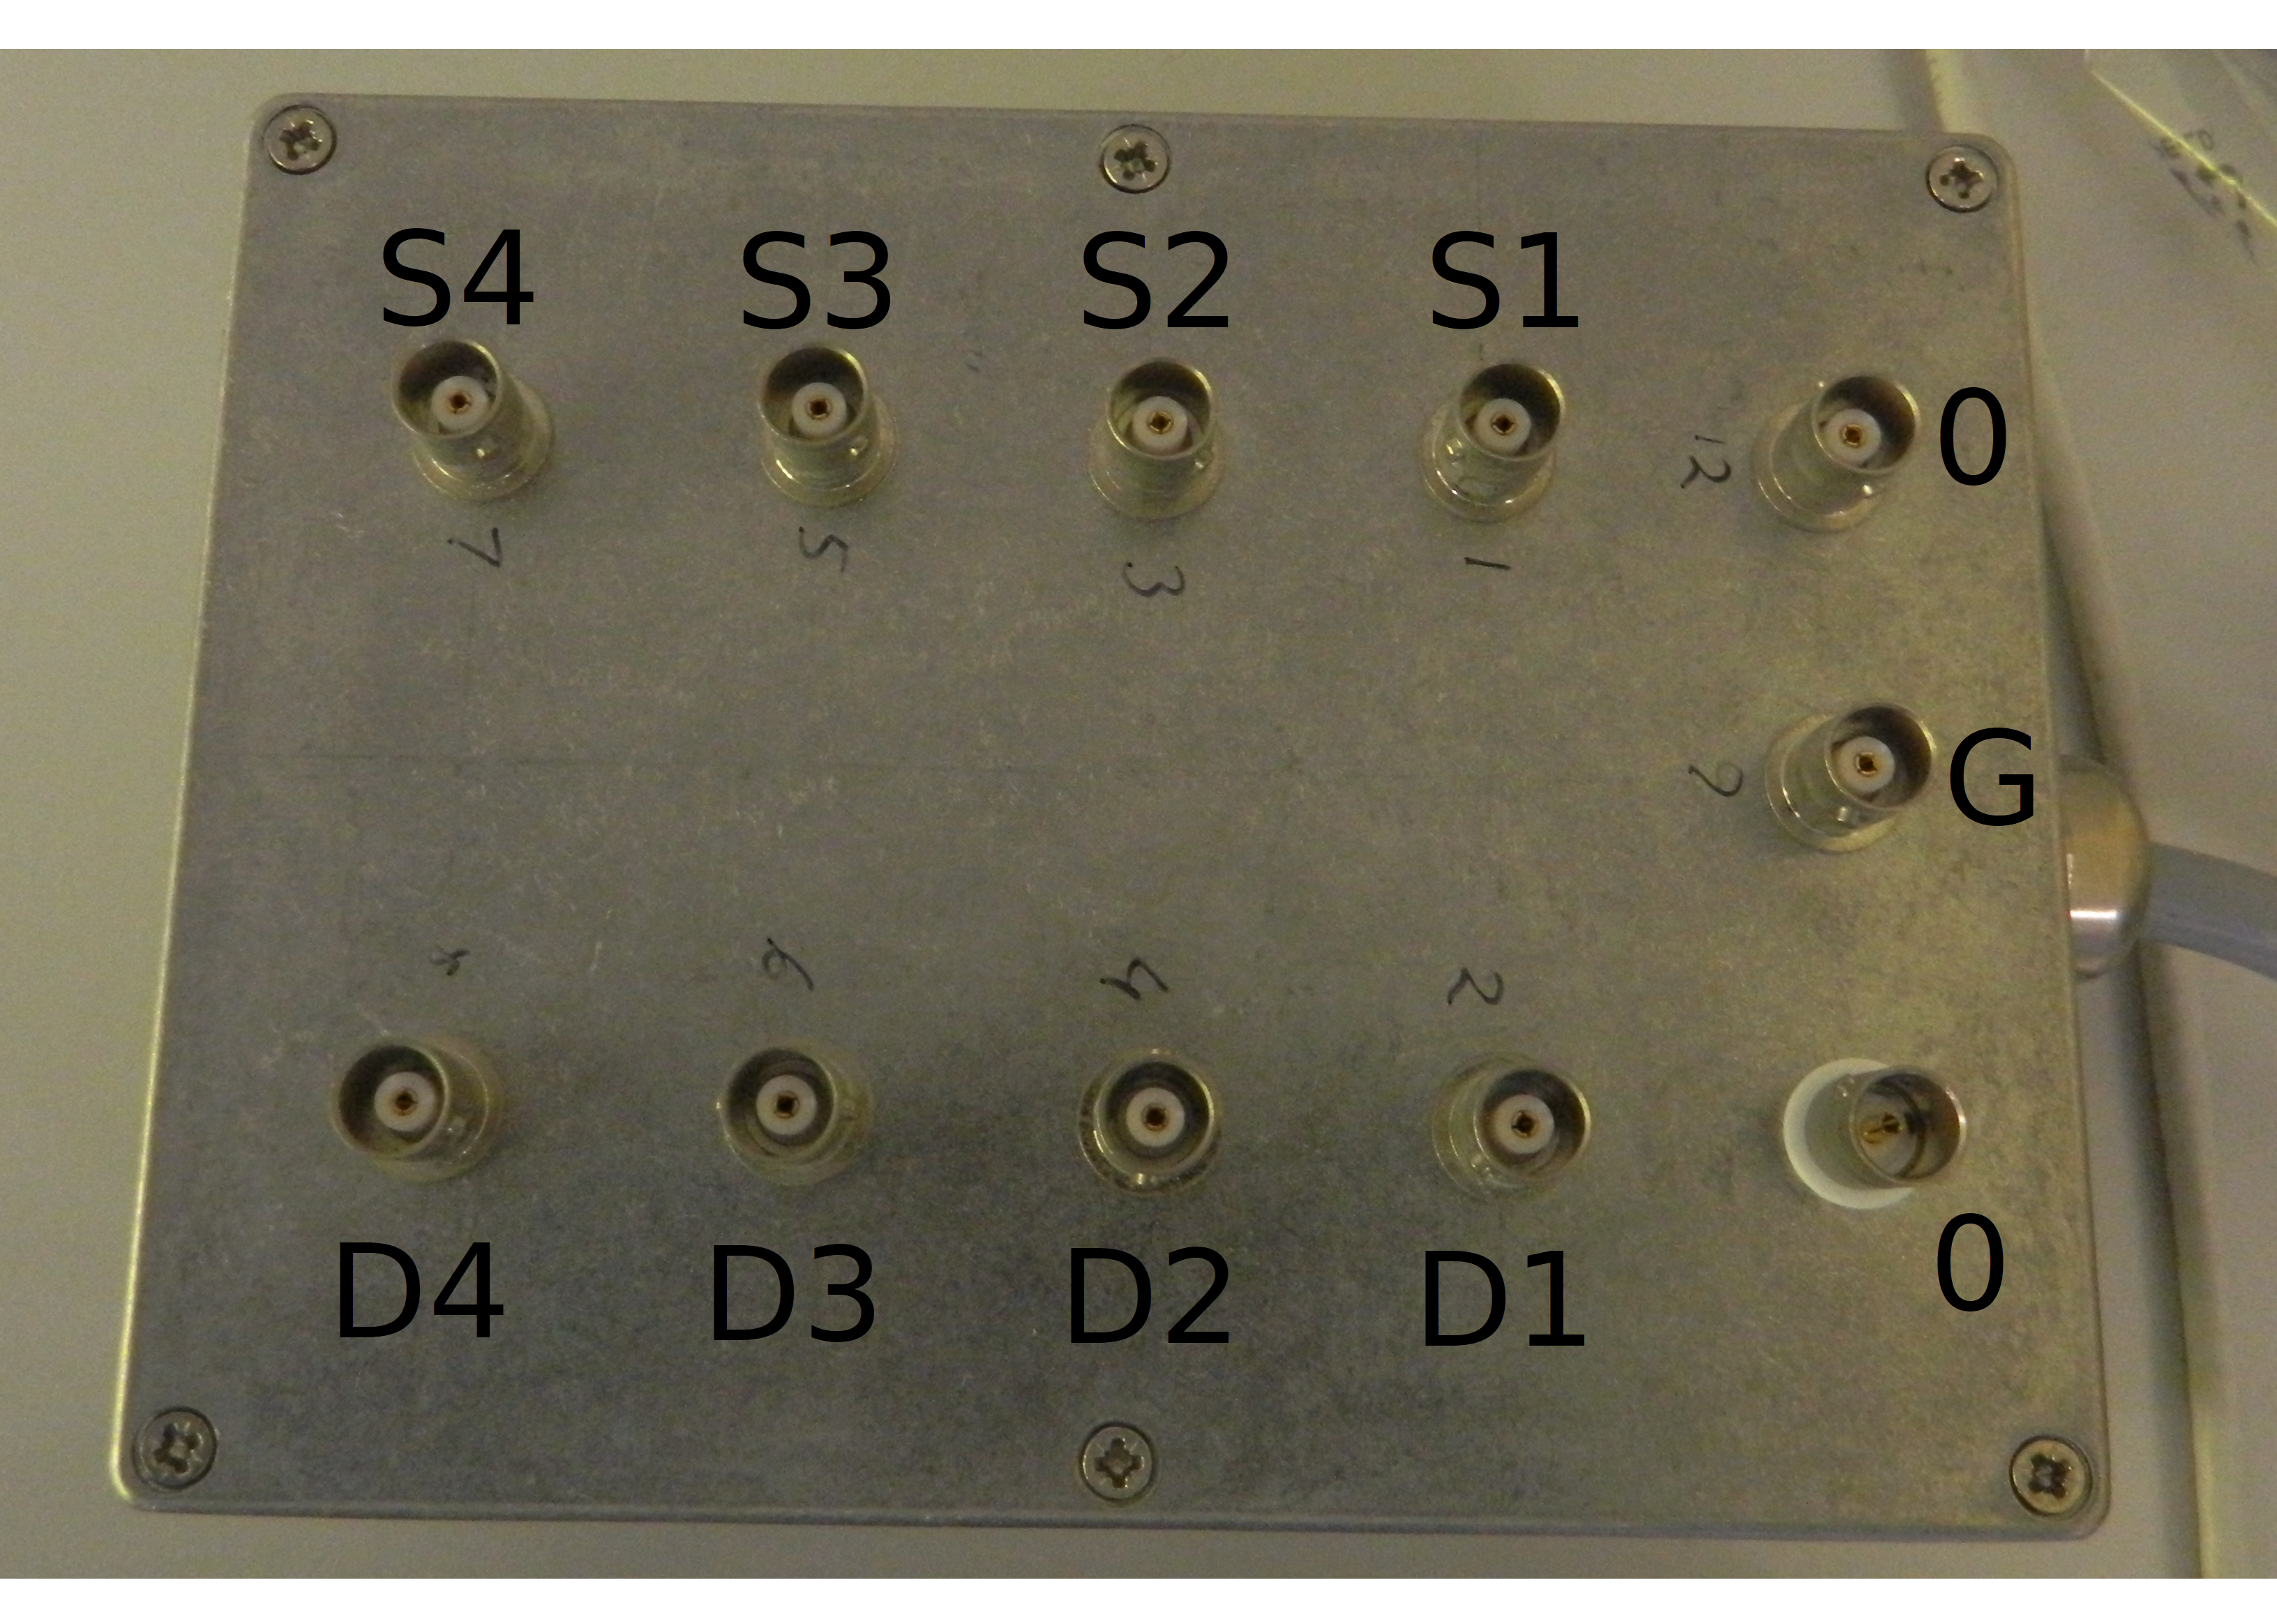
\includegraphics[width=0.65\textwidth,height=\textheight]{figures/ch10/multiplex-breakout.png}

}

\caption[Breakout board for multiplexing with a device inside the vapour
delivery system chamber.]{\label{fig-vapour-sensor-breakout}Breakout
board for multiplexing with a device inside the vapour delivery system
chamber. Source electrode terminals are labelled S, drain electrode
terminals are labelled D, the gate electrode terminal is labelled G and
disconnected terminals are labelled 0. Each number corresponds to a
different device channel.}

\end{figure}

Both setups should be sufficient for testing three iOR-functionalised
channels simultaneously alongside an empty iOR-functionalised channel.
To switch between analytes in a single vapour-phase sensing run with
uninterrupted flow, a second analyte bottle could be installed which
branches off from the existing carrier line. A solenoid-controlled 4-way
valve could be placed after these analyte bottles, which runs the vapour
flow from one analyte bottle to the exhaust and one into the chamber at
all times, as illustrated in
Figure~\ref{fig-vapour-sensor-multiplexing}.

\begin{figure}

{\centering \includegraphics[width=0.5\textwidth,height=\textheight]{figures/ch10/multiplex-vapoursensor.png}

}

\caption[Multiplexing with a second analyte bottle and four-way
valve.]{\label{fig-vapour-sensor-multiplexing}Multiplexing with a second
analyte bottle and four-way valve.}

\end{figure}

In this way, the amount of flow passing into the chamber is largely
unchanged across a sensing run. An advantage of this setup is that each
carrier line only ever contains one analyte to prevent
cross-contamination between lines. For multiplexing with more than two
analytes, more analyte bottles could be added and a 16-way or 32-way
valve used. This system could also be used to investigate the effects of
different exposure (sniff) times on the temporal resolution of sensing
devices \autocite{Spencer2021,Wu2024}.

\cleardoublepage
\phantomsection
\addcontentsline{toc}{part}{Appendices}
\appendix

\hypertarget{vapour-system-hardware}{%
\chapter{Vapour System Hardware}\label{vapour-system-hardware}}

\hypertarget{tbl-vapour-sensor-components}{}
\begin{longtable}[]{@{}
  >{\raggedright\arraybackslash}p{(\columnwidth - 4\tabcolsep) * \real{0.5930}}
  >{\raggedright\arraybackslash}p{(\columnwidth - 4\tabcolsep) * \real{0.2209}}
  >{\raggedright\arraybackslash}p{(\columnwidth - 4\tabcolsep) * \real{0.1860}}@{}}
\caption{\label{tbl-vapour-sensor-components}Major components used in
construction of the vapour delivery system described in this
thesis.}\tabularnewline
\toprule\noalign{}
\begin{minipage}[b]{\linewidth}\raggedright
Description
\end{minipage} & \begin{minipage}[b]{\linewidth}\raggedright
Part No.
\end{minipage} & \begin{minipage}[b]{\linewidth}\raggedright
Manufacturer
\end{minipage} \\
\midrule\noalign{}
\endfirsthead
\toprule\noalign{}
\begin{minipage}[b]{\linewidth}\raggedright
Description
\end{minipage} & \begin{minipage}[b]{\linewidth}\raggedright
Part No.
\end{minipage} & \begin{minipage}[b]{\linewidth}\raggedright
Manufacturer
\end{minipage} \\
\midrule\noalign{}
\endhead
\bottomrule\noalign{}
\endlastfoot
Mass flow controller, 20 sccm full scale & GE50A-013201SBV020 & MKS
Instruments \\
Mass flow controller, 200 sccm full scale & GE50A-013202SBV020 & MKS
Instruments \\
Mass flow controller, 500 sccm full scale & FC-2901V & Tylan \\
Analogue flowmeter, 240 sccm max. flow & 116261-30 & Dwyer \\
Micro diaphragm pump & P200-B3C5V-35000 & Xavitech \\
Analogue flow controller, for micro diaphragm pump & X3000450 &
Xavitech \\
10 mL Schott bottle & 218010802 & Duran \\
PTFE connection cap system & Z742273 & Duran \\
Baseline VOC-TRAQ flow cell, purple & 043-950 & Ametek Mocon \\
Baseline VOC-TRAQ flow cell, red & 043-951 & Ametek Mocon \\
Humidity and temperature sensor & T9602-5-A & Telaire \\
\end{longtable}

\hypertarget{python-code-for-data-analysis}{%
\chapter{Python Code for Data
Analysis}\label{python-code-for-data-analysis}}

The code used for general analysis of field-effect transistor devices in
this thesis was written with Python 3.8.8. Contributors to the code used
include Erica Cassie, Erica Happe, Marissa Dierkes and Leo Browning. The
code is located on GitHub and the research group OneDrive, as well as
being publicly available on Figshare \autocite{Treacher2024}.

\hypertarget{sec-histogram-analysis}{%
\section{Atomic Force Microscope Histogram
Analysis}\label{sec-histogram-analysis}}

The purpose of this code is to analyse atomic force microscope (AFM)
images of carbon nanotube networks in .xyz format (see
\textbf{?@sec-afm-characterisation}). It was originally designed by
Erica Happe in Matlab, and adapted by Marissa Dierkes and myself for use
in Python. The code imports the .xyz data and sorts it into bins 0.15 nm
in size for processing. To perform skew-normal distribution fits, both
\emph{scipy.optimize.curve\_fit} and \emph{scipy.stats.skewnorm} modules
are used in this code.

\hypertarget{sec-raman-analysis}{%
\section{Raman Spectroscopy Analysis}\label{sec-raman-analysis}}

The purpose of this code is to analyse a series of Raman spectra taken
at different points on a single film (see
\textbf{?@sec-raman-characterisation}). Data is imported in a series of
tab-delimited text files, with the low wavenumber spectrum (100
cm\(^{-1} - 650\) cm\(^{-1}\)) and high wavenumber spectrum (1300
cm\(^{-1} - 1650\) cm\(^{-1}\)) imported in separate datafiles for each
scan location.

\hypertarget{sec-field-effect-transistor-analysis}{%
\section{Field-Effect Transistor
Analysis}\label{sec-field-effect-transistor-analysis}}

The purpose of this code is to analyse electrical measurements taken of
field-effect transistor (FET) devices. Electrical measurements were
either taken from the Keysight 4156C Semiconductor Parameter Analyser,
National Instruments NI-PXIe or Keysight B1500A Semiconductor Device
Analyser as discussed in \textbf{?@sec-electrical-characterisation}; the
code is able to analyse data in .csv format taken from all three
measurement setups. The main Python file in the code base consists of
three related but independent modules: the first analyses and plots
sensing data from the FET devices, the second analyses and plots
transfer characteristics from channels across a device, and the third
compares individual channel characteristics before and after a
modification or after each individual modification in a series of
modifications. The code base also features a separate config file and
style sheet which govern the behaviour of the main code. The code base
was designed collaboratively by myself and Erica Cassie over GitHub
using the Sourcetree Git GUI.

\hypertarget{sec-vapour-delivery-analysis}{%
\section{Vapour Delivery System
Analysis}\label{sec-vapour-delivery-analysis}}

The purpose of this code is to display electrical measurements taken of
field-effect transistor devices inside the vapour delivery system
chamber alongside data collected from the photoionisation detector and
mass flow controllers. Electrical measurements were taken with the
Keysight 4156C Semiconductor Parameter Analyser or Keysight B1500A
Semiconductor Device Analyser, using the vapour sensing chamber chip
carrier described in \textbf{?@sec-electrical-characterisation}.
Electrical data is imported from a .csv file, while photoionisation
detector data is imported from a tab-delimited text file and mass flow
controller data is imported from a .lvm file.

\hypertarget{references}{%
\chapter*{References}\label{references}}
\addcontentsline{toc}{chapter}{References}

\markboth{References}{References}

\begingroup
\raggedright

\printbibliography[heading=none]

\endgroup

\newpage{}

\hfill\break

\thispagestyle{empty}

\mbox{~} \clearpage \newpage


\backmatter

\end{document}
